\chapter{Results} \label{chap:results}
\section{Validation and Verification}
Validation and Verification (V\&V) are needed to ensure that our code works as we expect. It is a necessary process in the field of computational simulations. They are essential for ensuring the reliability and accuracy of the simulation model. Verification is the process of confirming that a computational model accurately implements the intended mathematical model or theory. It checks that the simulation does what it's supposed to do mathematically and computationally.
It involves code verification (checking the code's or algorithm's accuracy) and solution verification (ensuring the solution is numerically accurate). Standard practices include checking against analytical solutions, performing grid convergence studies, and conducting code-to-code comparisons. Validation is the process of determining how well a computational model represents the real world. It is about assessing the accuracy of the simulation results in capturing the physical phenomena being modeled. This involves comparing simulation results with experimental or real-world data. It can include sensitivity analyses, uncertainty quantification, and benchmark cases. The aim is to demonstrate that the model can produce sufficiently accurate results for its intended application, ensuring the model's credibility in representing physical reality.

For complex simulations, such as turbulent flows or multi-physics problems, V\&V can be challenging due to the complexity of the phenomena and the need for exact analytical solutions.

We conducted three experiments to confirm that the implemented solver operates as expected:
\begin{itemize}
    \item \textbf{A falling sphere example, 1 phase}. Experiment with one phase and one solid body; in our case, it is a sphere. 
    \item \textbf{A bouncing sphere example, water-air}. Experiment with two phases and one solid body. The density of the body is smaller than one of the phases, which makes the body bounce and not sink.
    \item \textbf{A falling multi-spherical body}. This will show that a multispherical body in the shape of a sphere acts the same way as a simple sphere.
\end{itemize}

\subsection{A falling sphere example, 1 phase}
To initially validate the created numerical model of a single falling sphere, we conducted a comparative study between our one-phase falling sphere simulation and the results presented by Nan et al. (2023) \cite{nan2023high}. In their work, Nan et al. (2023) \cite{nan2023high} compared the numerical results of the drag coefficient simulation for different Reynolds numbers with experimental data. We utilized the same fluid and particle parameters in our simulation, as provided in Table \ref{table1-chap4_1}. Figure \ref{fig:1ph_exp_me} showcases the results obtained using the current \verb|cfdemSolverInterFlowIB| solver, alongside the simulation results from Nan et al. (2023) \cite{nan2023high}. A comparison of the velocity fields reveals that the fluid field around both particles is nearly identical. However, a visual comparison alone is insufficient for validation. Therefore, we also compared the velocity values and trajectory changes in the $z$-direction. The results of this comparison are presented in Figure \ref{fig:trajectory_1ph}.

\begin{table}[H]
    \centering
    \caption{Simulation Parameters} \label{table1-chap4_1}
    \begin{tabular}{llr}
        \toprule
        \hline
        Simulation Part         & Physical Parameters (units) & Value \\
        \hline
        \midrule
        Particle                 & Density (kg/m$^3$)          & 1200    \\
                         & Diameter (cm)          & 0.167    \\
                         & Initial height (cm)          & 3.5    \\
                         \hline
        Fluid                  & Density (kg/m$^3$)           & 1000   \\
                                & Viscosity (m$^2$/s)         & 1e$^{-6}$    \\
                                \hline
        \bottomrule
     \end{tabular}
\end{table}
%
%\begin{figure}[!ht]
%    \centering
%    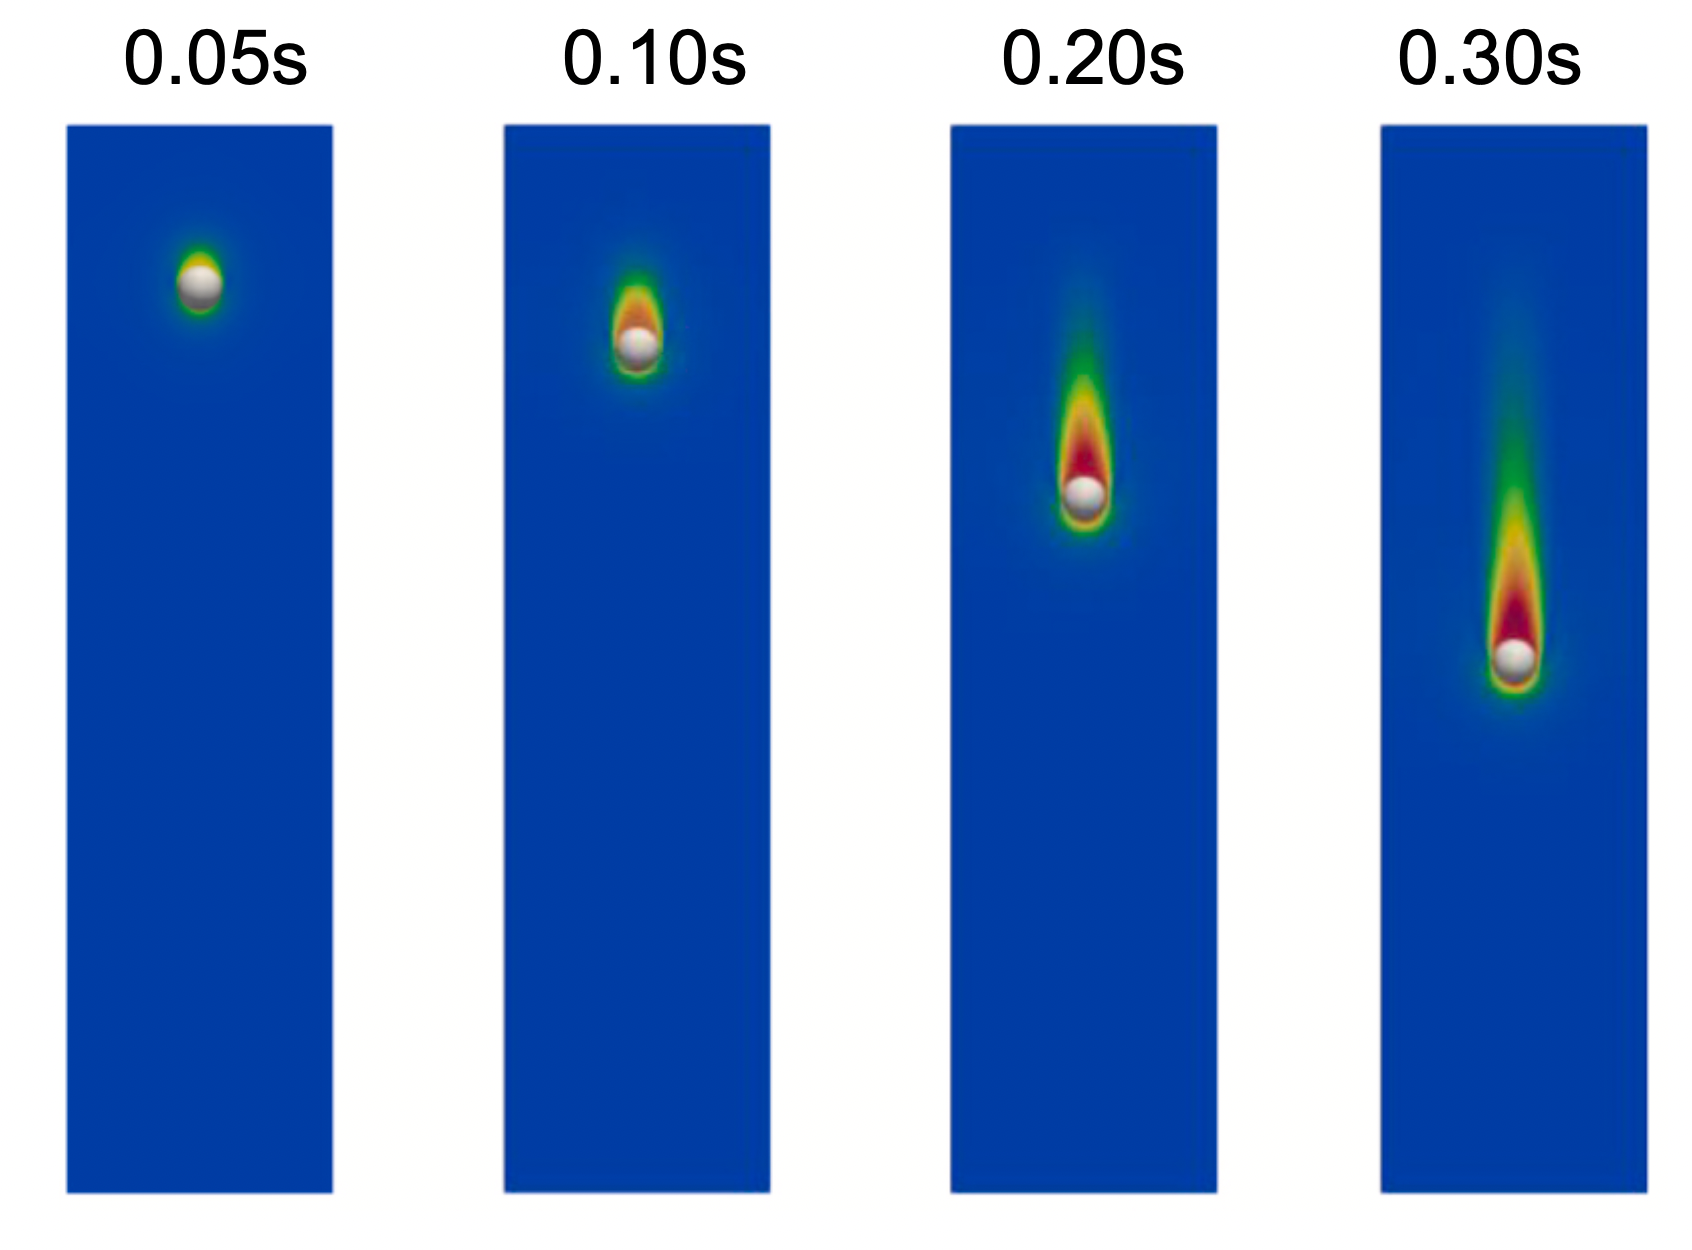
\includegraphics[width=10cm]{Images/chap3/1ph_exp.png}
%    \caption{Falling sphere simulation in 1 phase fluid from the work \cite{nan2023high}.}
%    \label{fig:1ph_exp}
%\end{figure}

\begin{figure}[!ht]
    \centering
    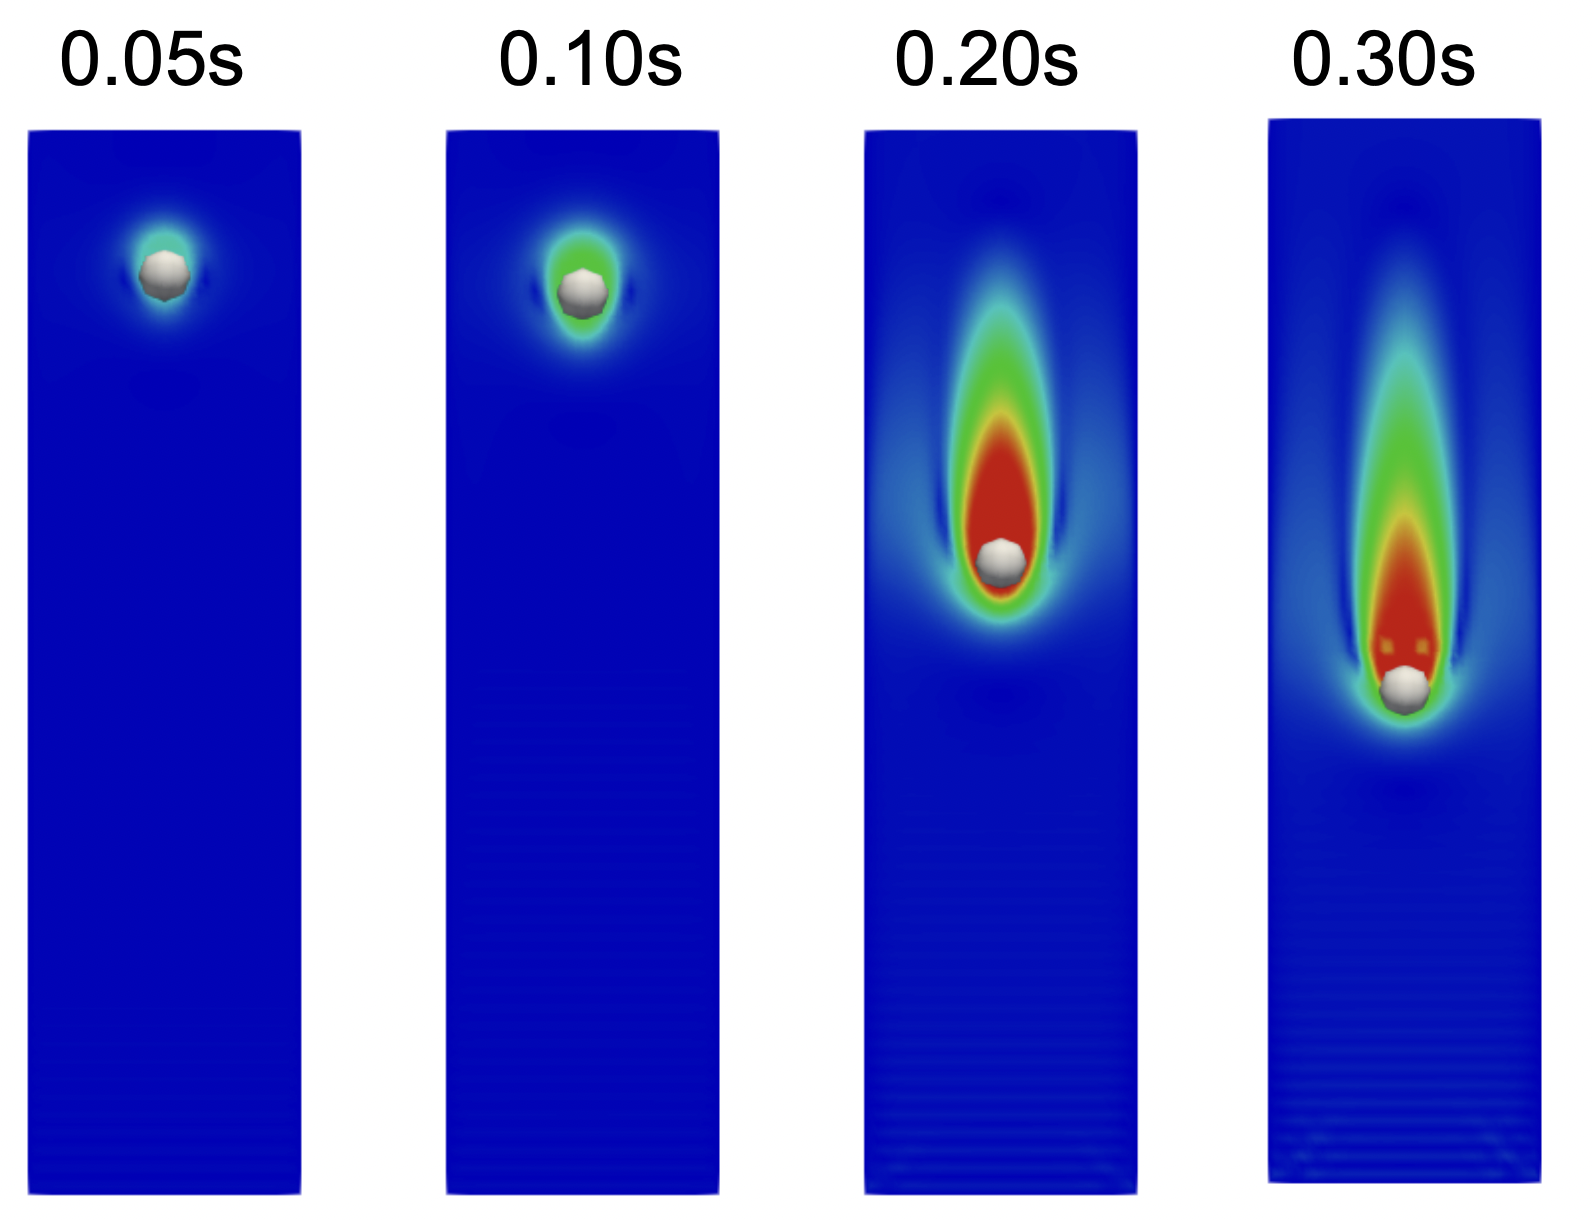
\includegraphics[width=10cm]{Images/chap3/1ph_exp_me.png}
    \caption{Velocity magnitude for falling sphere simulation in 1 phase fluid from the CFD-DEM simulation.}
    \label{fig:1ph_exp_me}
\end{figure}

More details are shown in Figure \ref{fig:trajectory_1ph}. The graph illustrates the trajectory and velocity comparison of a falling sphere in a one-phase fluid within our CFD-DEM simulation solver against the results published by Nan et al. (2023) \cite{nan2023high}. Both datasets present the time evolution of the sphere's $z$-direction movement and corresponding velocity. The plots are in good agreement with our simulation data (indicated by the orange dots) and the benchmark results from Nan et al. (2023)\cite{nan2023high} (represented by the solid black line) across the entirety of the simulated time-frame from 0 to 0.3 sec. This consistency in both position and velocity profiles supports our solvers' ability to accurately capture particle motion dynamics within a fluid. The variations observed are within acceptable ranges. The difference in the velocity field from 0 to 0.1 second may be attributed to the inherent discretization differences between the two simulation approaches. The difference between maximum velocities is $6$\%, which could stem from the nature of 3D simulation and because the observed order of convergence is 1. Despite that, we use the second-order method for CFD and DEM parts, and the mapping algorithm is first-order, which lowers the overall order of convergence.

The obtained data underscores the reliability of our CFD-DEM simulation and captures the essential physics of particle-fluid interaction.

\begin{figure}[!h]
    \centering
    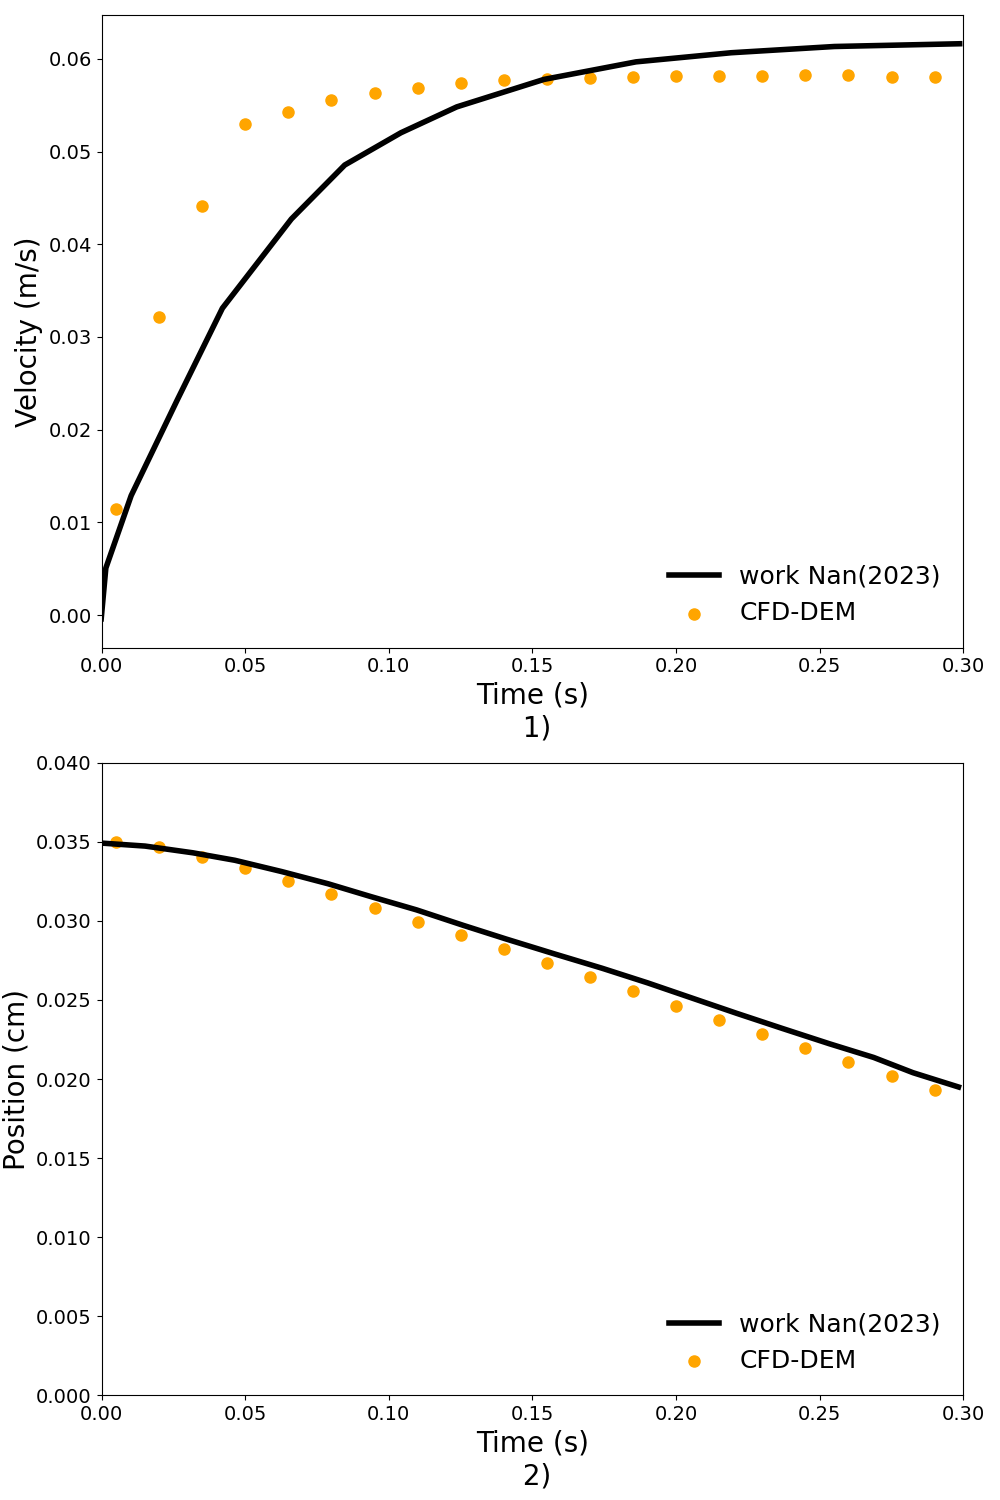
\includegraphics[width=13cm]{GWU_Thesis_Sarmakeeva/Images/chap3/nan_simulation_192000_cells_dt_0_0005_simulation.png}
    \caption{Falling sphere in 1 phase fluid 1) velocity of the particle 2) comparison in z-direction}
    \label{fig:trajectory_1ph}
\end{figure}

\newpage

\subsection{Grid convergence analysis.}

According to Roache's definition of code verification \cite{roache1998verification}, it means confirming the ability to solve the set of governing equations accurately. A main strategy for verifying the code is to conduct a grid convergence study, which involves executing multiple simulations on successive finer grids. The discretization error is expected to approach zero asymptotically as the grid is refined. The central point of interest in this context is the approximation order derived from the numerical method. For instance, if a second-order accurate method is used, we anticipate observing second-order convergence. However, in most cases, the second-order accuracy from spatial discretization can not be reached for two-way coupling problems, as stated in the paper Taira et al. (2007)\cite{taira2007immersed}.

Because we do not know the exact solution for the falling sphere simulation, we could apply Richardson extrapolation, which would be the best possible solution verification to measure discretization error.

The basic concept of  Richardson extrapolation was introduced in his work Richardson~(1911)~\cite{richardson1911}. If the formal rate of convergence of a discretization method with mesh refinement is unknown, but discrete solutions on two systematically refined meshes are available, then this information could be used to estimate the exact solution of a mathematical model. It could be used either to correct the fine mesh solution or to provide a discretization error estimate for it. Although Richardson initially developed the extrapolation approach for locally approximating the dependent variables within the mathematical model's domain, it can be conveniently extended to estimate any system response quantity. However, this extension comes with an additional prerequisite – the numerical approximations (such as integration, differentiation, etc.) employed to calculate the system response quantity must possess at least the same order of accuracy as the underlying discrete solutions.

The process of generalized Richardson extrapolation is described in a book by Oberkampf et al. \cite{oberkampf}. The generalized Richardson $\bar{f}$ could be found as:

\begin{equation}
\bar{f}=f_h+\frac{f_h-f_{r h}}{r^p-1}
\end{equation}
where $h$ is representative coarse mesh size and $rh$ is fine mesh. $f_h$ and $f_{rh}$ numerical solutions with mesh spacing $rh$, $p$ is the order of convergence. The grid refinement factor $r$ is the ratio of the coarse to fine grid spacing calculated as:
\begin{equation}
r=\frac{h_{\text {coarse }}}{h_{\text {fine }}}>1
\end{equation}

\begin{figure}[!ht]
    \centering
    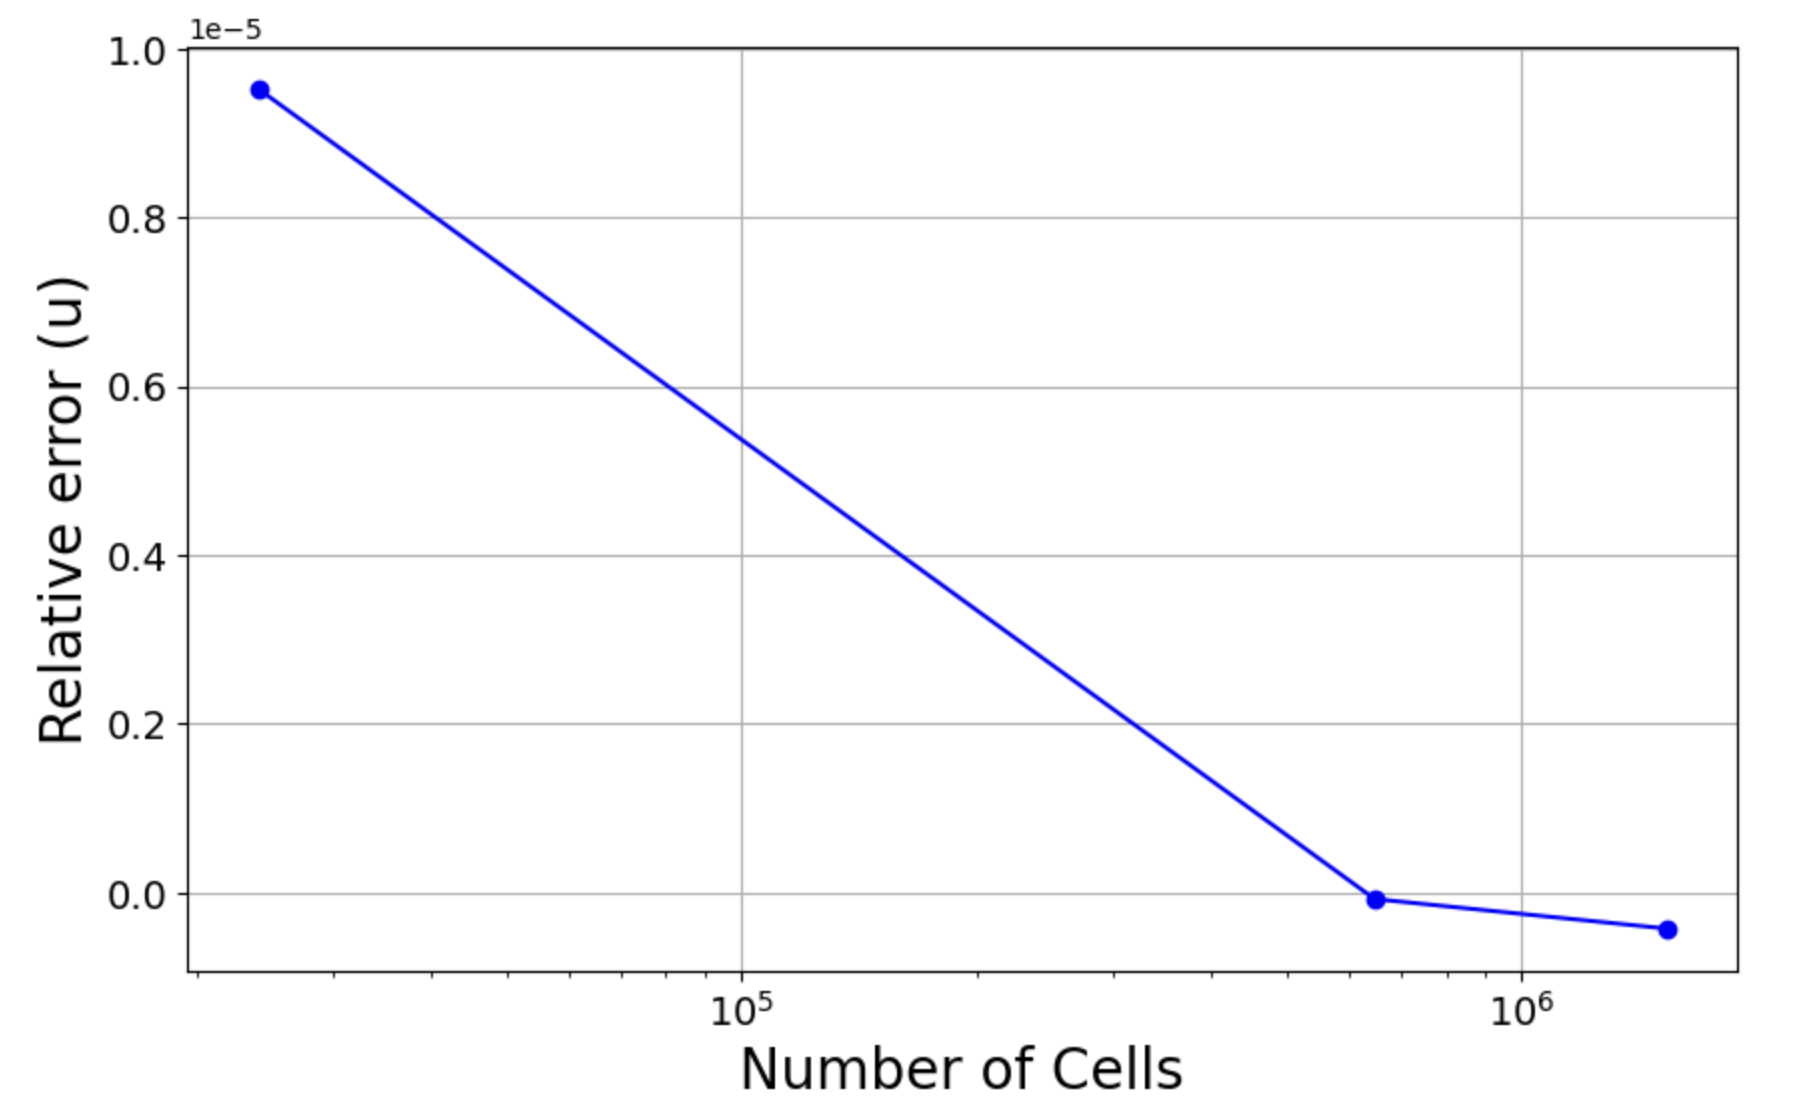
\includegraphics[width=16cm, height = 10cm]{GWU_Thesis_Sarmakeeva/Images/chap3/richardson_extrapoltation.png}
    \caption{The velocity relative error obtained for the problem of a 3D falling sphere with CFDEMcoupling, for implemented solver with introduced a coupling force model.}
   \label{fig:l2}
\end{figure}

By applying Richardson extrapolation, we found that the relative error for the finest mesh used in our simulations is on the order of magnitude $10^{-6}$. In engineering applications, the acceptable level of error is often determined by engineering judgment, considering factors such as the problem's complexity, the intended use of the solution, and the potential consequences of inaccuracies. Based on our understanding of the problem and the requirements for the solution, we have determined that a relative error of $10^{-6}$ is satisfactory for our purposes.
%When the exact solution is available, commonly used evaluation metric  is the $L_2$ er Euclidean norm, which is the root mean square of the error and for uniform mesh could be found as:
%\begin{equation}
%\left\|u-u_{\mathrm{ref}}\right\|_2=\left(\frac{1}{N} \sum_{n=1}^N\left|u_n-%u_{\mathrm{ref}, n}\right|^2\right)^{1 / 2}
%\end{equation}

%Another metric that we could use is $L_{\infty}$ infinity norm, which measures the maximum absolute error over the entire domain. It could be calculated as:

%\begin{equation}
%\left\|u-u_{\text {ref }}\right\|_{\infty}=\max \left|u_n-u_{\text {ref }, n}\right|, \quad n=1 \text { to } N
%\end{equation}


%\begin{figure}[!ht]
%    \centering
%    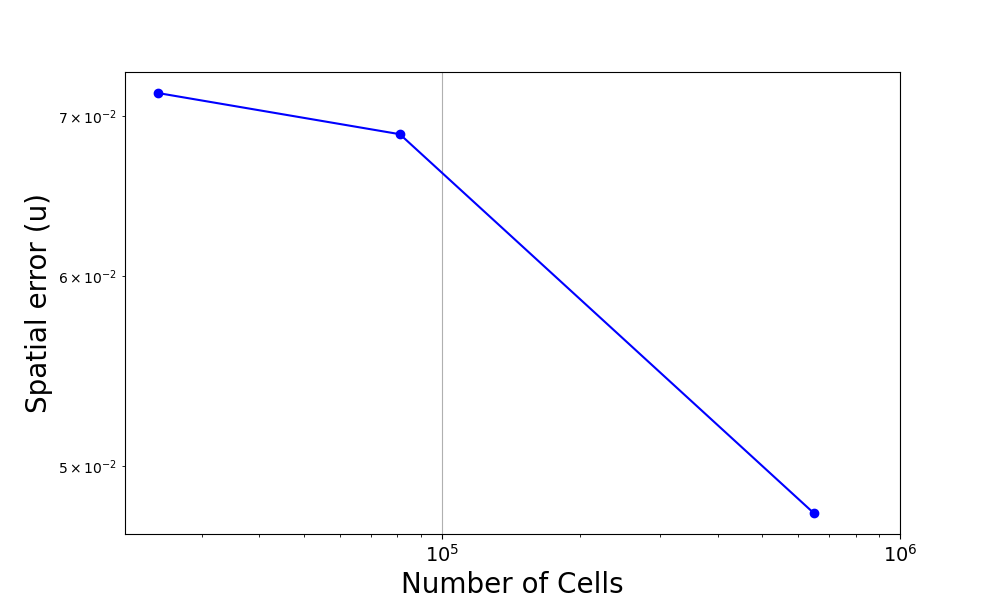
\includegraphics[width=16cm, height = 10cm]{GWU_Thesis_Sarmakeeva/Images/chap3/l2_norm.png}
%    \caption{$L_2$ norm of the velocity error obtained for the problem of a 3D falling sphere with CFDEMcoupling, for implemented solver with introduced a coupling force model.}
 %   \label{fig:l2}
%\end{figure}

%\begin{figure}[!ht]
 %   \centering
 %   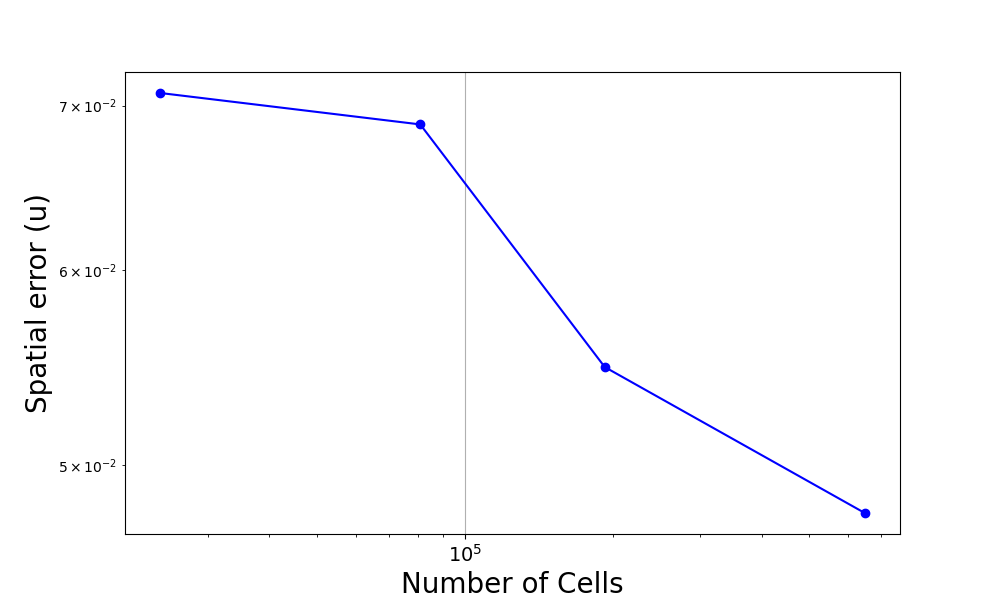
\includegraphics[width=16cm, height = 10cm]{ GWU_Thesis_Sarmakeeva/Images/chap3/l_inf.png }
%    \caption{$L_{\infty}$ norm of the velocity error obtained for the problem of a 3D falling sphere with CFDEMcoupling, for implemented solver with introduced a coupling force model.}
 %   \label{fig:l_inf}
%\end{figure}

%The graphs provided on Figure \ref{fig:l2}, and Figure \ref{fig:l_inf} represent the grid convergence study for a falling sphere simulation, showing how the average norm of velocity changes with the number of cells in the computational grid. 

%Figure \ref{fig:l_inf} displays the $L_{\infty}$ norm of velocity error against the number of cells. The trend indicates that as the number of cells increases, the maximum velocity magnitude across the domain initially decreases sharply and then levels off, suggesting that a grid-independent solution is being approached. The plateau in the curve suggests that further refinement of the grid does not significantly change the maximum velocity, indicating that convergence has been reached for this norm.

%The second graph, Figure \ref{fig:l2}, shows the $L_2$ norm of velocity error against the number of cells. Similar to the $L_{\infty}$ norm results, the graph shows a decrease in the average $L_2$ norm as the number of cells increases, with the rate of decrease diminishing as the number of cells becomes large. This suggests that the solution is approaching grid independence, where further refinement does not lead to significant changes in the overall velocity field as perceived by the $L_2$ norm.
Further insights from a grid-convergence study reveal an improvement in scheme accuracy with an increased cell count, underscoring the importance of grid refinement in simulation accuracy. The findings suggest that careful consideration of the exchange time step frequency and grid resolution is important for optimizing solver performance and ensuring the reliability of the simulation results.

The implemented algorithm has different communication times as part of a two-way coupling process. For example, we would do ten iterations of the DEM algorithm and then send the force and positions of particles to CFD. It could be useful to save computational resources. The common practice is to set up communication between DEM and CFD solutions every $5$th or $10$th computational step, which means that the time-step for the DEM part $10$ time would be smaller than for the OpenFOAM solver.

To better understand how these parameters could affect the computations, we completed an analysis running a falling sphere simulation for different settings of different communication times of coupled parts. Results are provided in Figure \ref{fig:communication} below.

\begin{figure}[!h]
    \centering
    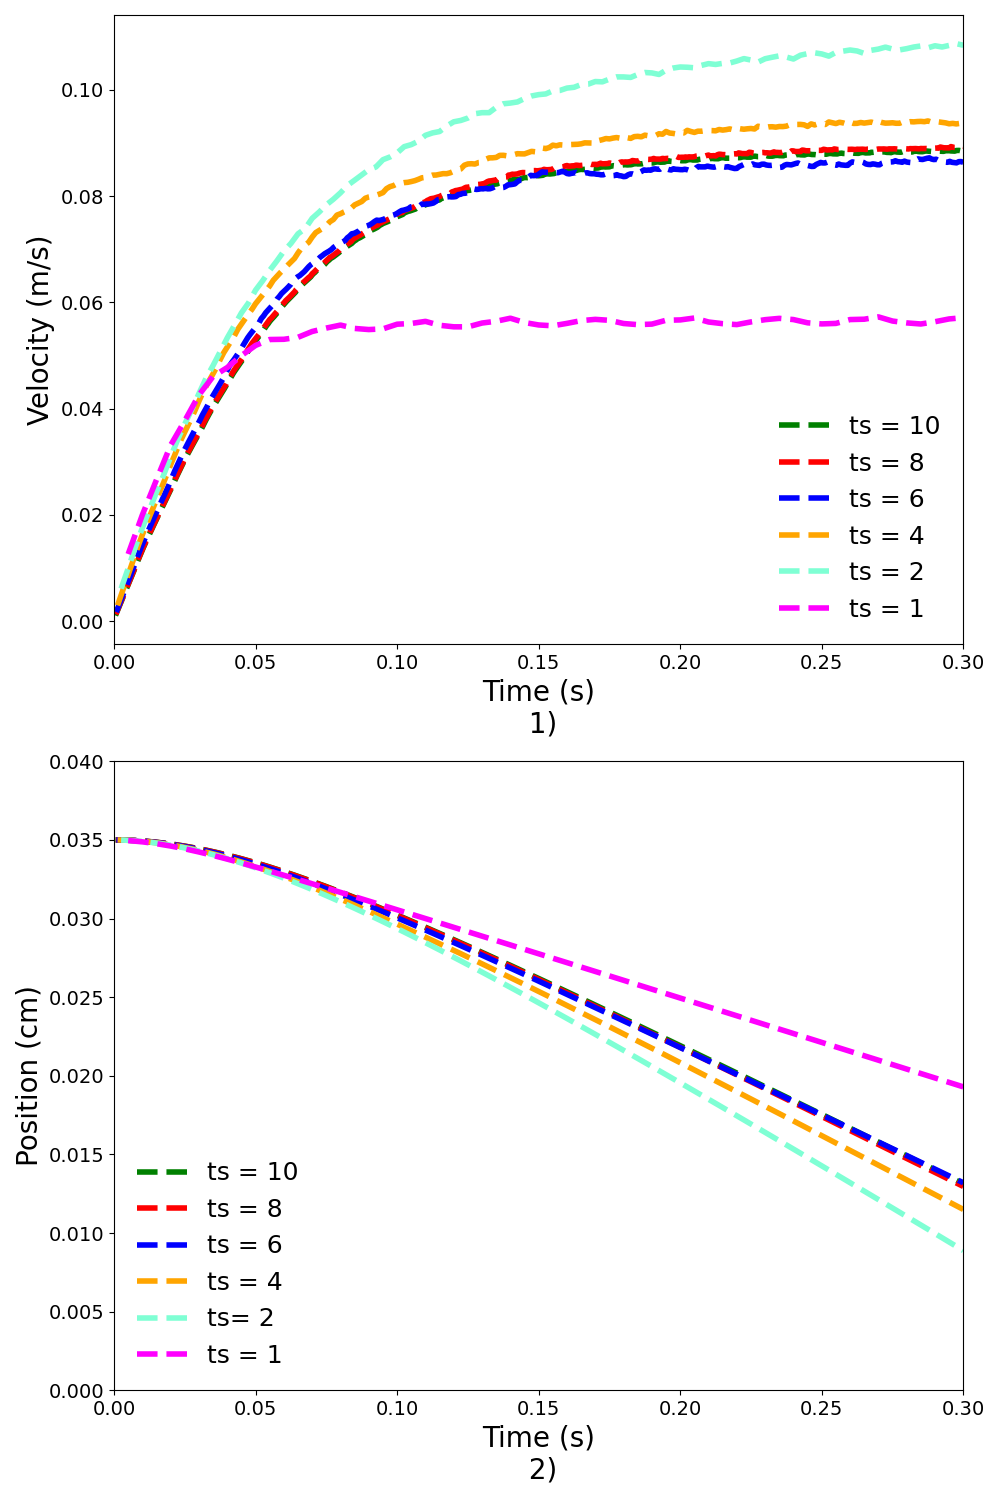
\includegraphics[width=13cm]{ GWU_Thesis_Sarmakeeva/Images/chap3/nan_simulation_192000_diff_exchange_time.png}
   \caption{Different settings for communication between CFD and DEM parts for every 10, 8, 6, 4, 2, 1 exchange time step  $ts$ 1) velocity component 2) change in z-direction .}
    \label{fig:communication}
\end{figure}

Figure \ref{fig:communication} shows the data for the problem of a 3D falling sphere with CFDEMcoupling. It is implemented as a solver for the coupling DEM and CFD part incorporating the force model. Which means how we exchange and apply forces to each part of the simulation. On Figure \ref{fig:communication} $ts$ is the time step for data exchange. CFD and DEM solvers communicate every 10th, 8th, 6th, 4th, 2nd, and each computational step correspondingly. Figure \ref{fig:communication} shows that different exchange steps affect the sphere's velocity and position, highlighting the critical role of exchange time step frequency in the numerical stability of the coupled scheme. Notably, a discrepancy in velocity is observed when comparing exchange steps $1$ and $2$. The velocity results that we got for exchange time $1$ are similar to velocity from the work of Nan et al. (2023)\cite{nan2023high}, while velocity for other exchange time steps is significantly overestimated.

\begin{figure}[H]
    \centering
    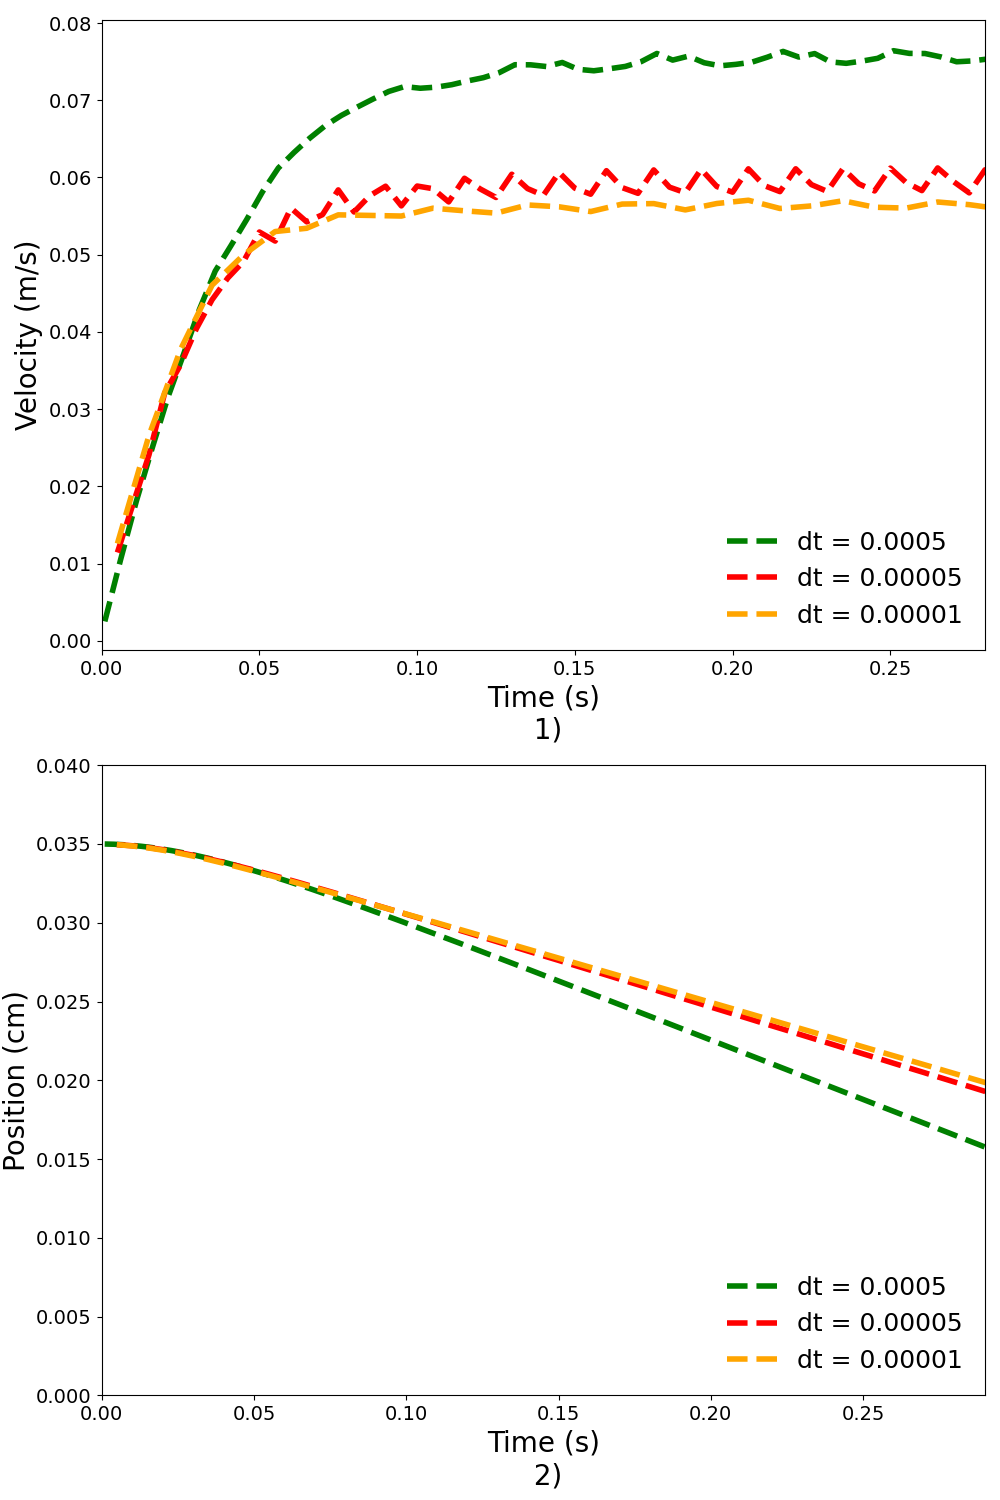
\includegraphics[width=12cm]{ GWU_Thesis_Sarmakeeva/Images/chap3/nan_simulation_192000_cells_dt_different.png }
    \caption{ Different setting for $\Delta t$ 1) velocity component 2) change in z-direction.}
    \label{fig:diff_dt}
\end{figure}

Another simulation done where there were computations of 3D falling spheres for the different time steps. Results for $\Delta t = 0.00001$, $0.00005$ and $0.0005$ are shown on Figure \ref{fig:diff_dt}. For this experiment, we used a mesh with 192000 computational cells.
\begin{figure}[H]
    \centering
    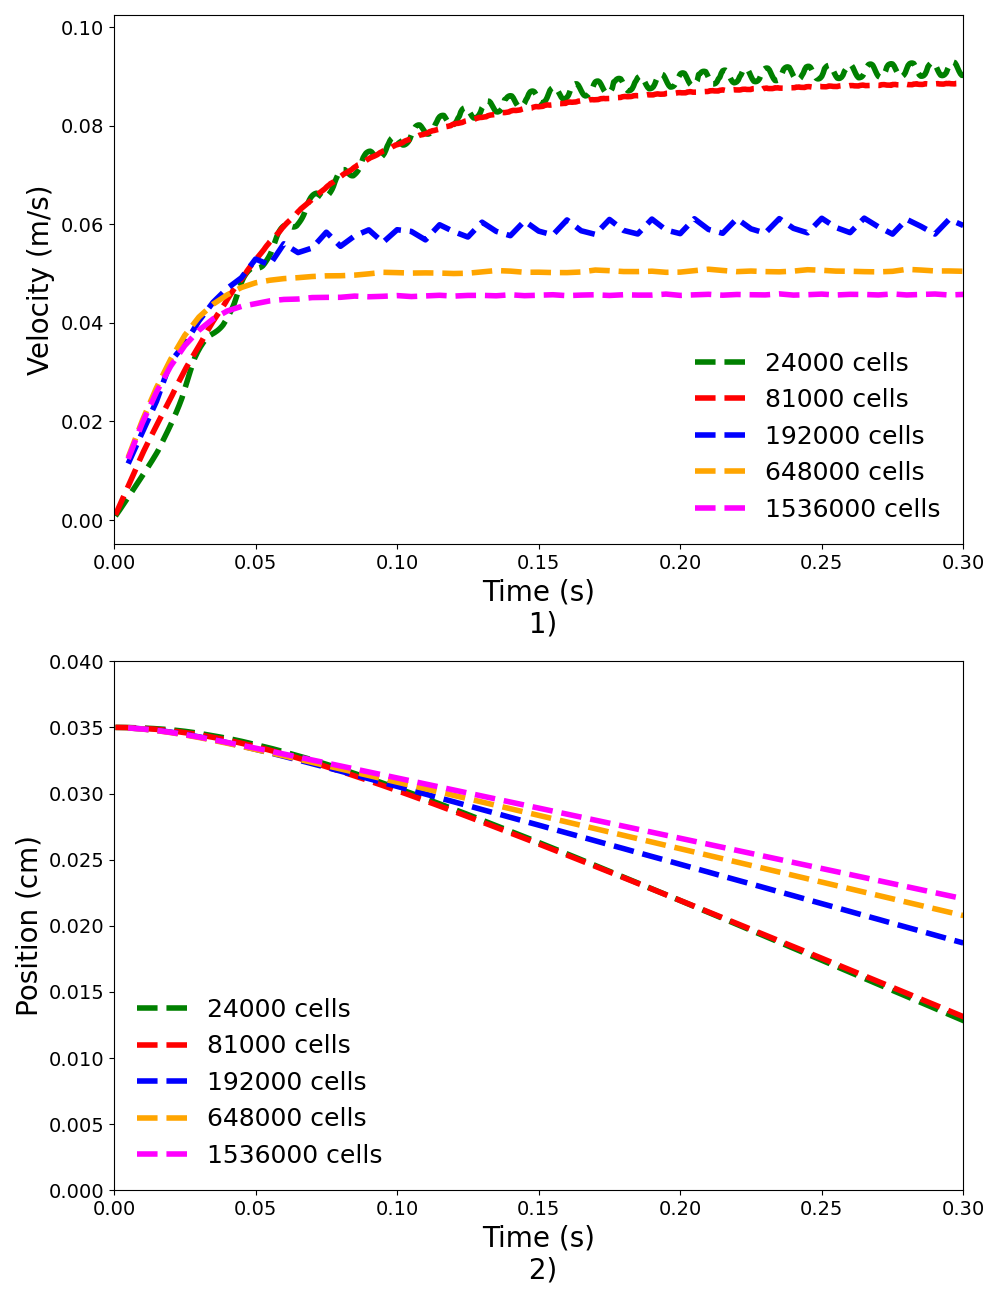
\includegraphics[width=14cm]{ GWU_Thesis_Sarmakeeva/Images/chap3/nan_simulation_192000_diff_cells_number.png}
    \caption{A different setting for $\Delta x$: 1) velocity component 2) change in the z-direction.}
    \label{fig:cell_num}
\end{figure}
As we can see from the results for the velocity change, $\Delta t = 0.0005$ oscillates, but for $\Delta t = 0.00001$ and $0.00005$ oscillations insignificant; however, there is an overestimation in velocity for $\Delta t = 0.00005$. For the smallest time step $\Delta t = 0.00001$, we see that the maximum velocity value is close to $0.6$ m/s, which corresponds to results provided in Figure~\ref{fig:trajectory_1ph}. Then, we run experiments for different numbers of computational cells.

To calculate the spatial error, we run the simulation with refinement factor $1.5$ for different numbers of computational cells, parameters of the meshes provided in Table \ref{table1-chap4}:

\begin{table}[H]
    \centering
    \caption{Mesh Parameters for calculation spatial error. } \label{table1-chap4}
    \begin{tabular}{llll}
        \toprule
        \hline
        Name     & Cell number & dimensions&$x\times y \times z $\\
        \hline
        \midrule
        Mesh 1   & 24000 && 20 20 60\\
        Mesh 2 & 81000 & &30 30 90\\
        Mesh 3 & 192000 &&40 40 120 \\
        Mesh 4 & 648000 & &60 60 180 \\
        Mesh 5 & 1536000 & &80 80 240\\
        \hline
        \bottomrule
     \end{tabular}
\end{table}

In Figure \ref{fig:cell_num}, we observe the simulation results that correlate with the number of computational cells used in the mesh. The results of the coarser meshes with 24000 and 192000 cells exhibit oscillations, as evidenced by the overestimation in the velocity data and position of the change in $z$-direction underestimates. For 192000 cells, results are close to the experiment Nan et al. (2023) \cite{nan2023high}, but we still can observe oscillations in the velocity results. Conversely, the mesh with 81,000 cells yields more stable outcomes, yet there remains a notable deviation from the results obtained with higher-resolution meshes, indicating potential inaccuracies. This difference could be a consequence of the mapping algorithm used for calculations, as discussed in the work by Nan et al. (2023) \cite{nan2023high}, because they also observed oscillations in results.

As the mesh is refined from coarser resolutions to 648,000 and 1,536,000 cells, the simulation results exhibit improved accuracy and a trend toward convergence. The close agreement in $9$\% between the solutions obtained on these two higher-resolution meshes suggests that the numerical solution is approaching an asymptotic state, where further mesh refinement would not significantly alter the results, especially for an observed order of convergence of 1. Conducting simulations with an excessively large number of computational cells may be impractical because the simulation of over a million computational cells takes more than 24 hours. Increasing the cell count beyond a certain threshold will likely yield diminishing returns in terms of accuracy while significantly increasing the computational resources and time required. This asymptotic behavior, known as a mesh-independent solution, is an indicator of numerical convergence.

Numerical convergence is a critical aspect of CFD simulations, as it demonstrates that the discretized equations and numerical methods employed in the solver are capable of accurately representing the underlying governing equations and physics of the problem. When a mesh-independent solution is achieved, it implies that the numerical errors introduced by the discretization process have been minimized to an acceptable level, and the solution can be considered a reliable approximation of the true, continuum solution.

The observation that discrepancies in the solutions are more pronounced on coarser meshes, while the higher-resolution meshes exhibit close agreement, suggests that the mesh resolution plays a crucial role in capturing the flow features accurately. This behavior may result from the interaction between the mesh resolution and the mapping algorithm used to discretize the governing equations onto the computational CFD mesh. 

%By systematically refining the mesh and observing the convergence of the solution, we can establish confidence in the numerical results and quantify the discretization errors associated with a given mesh resolution. This process is often referred to as a mesh convergence study and is an essential step in verifying the numerical accuracy and reliability of CFD simulations.

\section{The two-phase experiments.}

In a subsequent validation phase, we run two experiments. One is a sphere falling into the water and bouncing on the free surface, where results are compared with the work of Pathak et al.~ (2016) \cite{pathak20163d}. We test this experiment to compare and see that simulation is converging and gives similar results as in the work Pathak et al. (2016) \cite{pathak20163d}, which is compared with the physical experiment.
The second simulation extended, including a multi-spherical body that consists of 2 spheres. This experiment assessed the solver's capability to interact with the free surface with complex particle shapes while maintaining the same fluid and particle parameters outlined in Table \ref{table3-chap4}.

\begin{table}[H]
    \centering
    \caption{Simulation Parameters} \label{table2-chap4}
    \begin{tabular}{llr}
        \toprule
        \hline
        Simulation Part         & Physical Parameters (units) & Value \\
        \hline
        \midrule
        Particle                 & Density (kg/m$^3$)          & 500    \\
                         & Diameter (cm)          & $0.252$    \\
                         & Initial height (cm)          & $1.0252$    \\
                         \hline
        Fluid                  & Density (kg/m$^3$)           & $1000$   \\
                                & Viscosity (m$^2$/s)         & 1e$^{-6}$    \\
                                \hline
         Air                  & Density (kg/m$^3$)           & $1e-5$   \\
                                & Viscosity (m$^2$/s)         & 1e$^{-6}$    \\
                                \hline
        \bottomrule
     \end{tabular}
\end{table}
Figures \ref{fig:two-phase_sphere} and \ref{fig:IB} present the simulation outcomes for a sphere from the published work Pathak et al. (2016) \cite{pathak20163d} and our solver, respectively. Results show good agreement, for the maximum velocity the difference is less than 6\% and for the average velocity the difference is around 25\%. For a more quantitative insight, Figure \ref{fig:2ph_exp} displays the trajectory in the $z$-direction of the falling sphere.

\subsection{A bouncing sphere example, water-air}
The initial experiment comes from the work Beck et al. (1897) \cite{beck1987transient} where they use the tank parameters: length: 109.7 m, width 6.7 m, depth 3.2 m. The sphere radius $r= 0.254$ m, height $z = r/10$ above the free surface. The sphere density is 500 kg/m.

First, we tried to make a regular mesh similar to the work of Pathak et al. (2016) \cite{pathak20163d} work. For the domain size from Pathak etc.\cite{pathak20163d} we followed formula:
\begin{equation}
    (length \cdot height \cdot width)  \cdot  r  \cdot  CPR,
\end{equation}
where CPR - cell per radius of the sphere. To save computational resources for tank size of $13\times 6.7 \times 3.4$ $\approx 17$ M cells with CPR $= 10$ $\approx 8$ M cells for tank $5\times 5 \times 5$, CPR~$=~10$~$\approx~2.7$~M cells for tank $5\times 5 \times 5$ with mesh refinement to the center, CPR~$= 10$

The CPR~$= 10$ mesh resolution results of the simulation are shown in Figure \ref{fig:2ph_exp}. Where by the red line represents results with the current solver, the black line shows results from Pathak et al. (2016) \cite{pathak20163d}, and the blue line results from the physical experiment Beck and Liapis (1987)\cite{beck1987transient}.
\begin{figure}[!ht]
    \centering
    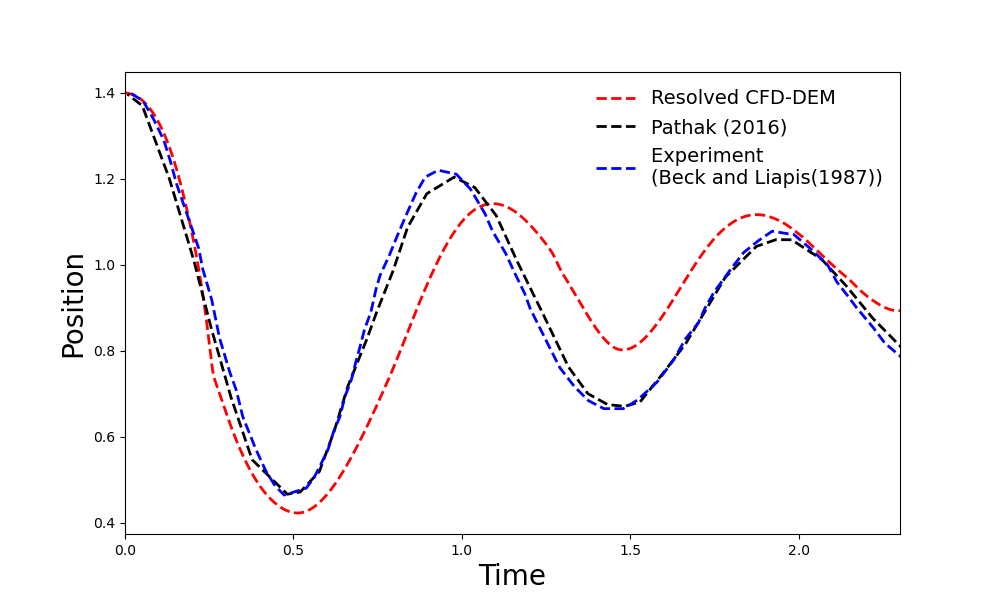
\includegraphics[width=15cm]{Images/chap3/bouncing_sphere_plot.png}
    \caption{Bouncing sphere simulation for two-phase fluid from the CFD-DEM simulation. The red line is the results with the current solver; the black line is the results from Pathak et~al.~(2016) \cite{pathak20163d}, the blue line is the results from the physical experiment by Beck and Liapis~(1987)~\cite{beck1987transient}.}
    \label{fig:2ph_exp}
    \end{figure}
    
The main parameters are shown in Table \ref{table2-chap4}. Given the complexity of the two-phase falling sphere simulation, increasing the number of computational cells beyond a certain point may not be the most efficient approach. Average velocity differs by $25$\% and maximum velocity $5$\%. This difference can be attributed to the inherent complexity of 3D simulations and the observed first-order convergence of the overall method. Although second-order methods are employed for both the CFD and DEM components of the simulation, the mapping algorithm connecting these two parts is first-order accurate. Consequently, the overall order of convergence is reduced, leading to the observed variation in maximum velocities. Despite this difference, the 5\% discrepancy in maximum velocities is considered acceptable within the context of the simulation's objectives and the limitations imposed by the coupling algorithm. In future work, the development of higher-order mapping algorithms could be explored to improve the overall order of convergence and further reduce the differences in maximum velocities. 

Our current computational resources would require more than 24 hours to complete the simulation with a significantly higher cell count. While finer mesh resolutions can improve accuracy, the substantial increase in computational time might not justify the marginal gains in precision. Finding a balance between simulation accuracy and computational feasibility is important to ensure that we can obtain reliable results within a reasonable time-frame while also being mindful of the efficient utilization of our computational resources. The current simulation setup provides valuable insights into the system's behavior and serves as a foundation for further refinement and analysis.

Figure \ref{fig:two-phase_sphere} provides a series of time-step snapshots from a CFD-DEM simulation of a sphere interacting with a two-phase fluid, where dark blue is a liquid with the density of water and light blue is a liquid with the density of the air.

\begin{itemize}
    \item \textbf{Initial Contact (a - 0.1 sec):} The sphere is shown just above the fluid interface, moving under gravity force in the direction of the water
    \item \textbf{Entry and Deformation (b - 0.2 sec):} As the sphere impacts the fluid surface, we see the beginning of deformation at the fluid interface, indicating the sphere's entry into the water. The fluid is distorted in response to the sphere's presence, which illustrates the initial splash or the beginning of the sphere's submersion.
    \item \textbf{Submersion and Displacement (c - 0.4 sec):}The sphere is now submerged, and we can observe the water deforming significantly around the sphere, due to water displacement as the sphere moves downward. The scheme is converging even under significant changes in free surface.
    \item \textbf{Maximum Penetration (d - 0.7 sec):} This image might represent the sphere at or near its maximum depth, given the substantial fluid displacement.
    \item \textbf{Upward Motion (e - 0.9 sec):} The sphere is moving upward, indicating that it is buoyant as indicated by the changing flow patterns and the 'tail' of disturbed fluid below it.
    \item \textbf{Surface Re-contact (f - 1.2 sec):} The sphere has ascended back to the fluid interface, and we can see the water's surface is deformed as the sphere pushes up against it, about to break through the surface again.
\end{itemize}

This simulation is essential to test the numerical accuracy of the algorithm for surface tension calculation of the numerical scheme, and experiments confirm its validity. By comparing the simulation results with experimental data, we can assess the ability of the numerical scheme to accurately capture the complex dynamics of surface tension in multiphase flows. The agreement between the simulated and experimental results provides confidence in the overall reliability of the numerical model. Furthermore, this validation process helps identify potential limitations and areas for improvement in the numerical scheme, enabling us to refine and optimize the model for more accurate and efficient simulations of surface tension-driven phenomena in various applications.
\begin{figure}[H]
    \centering
    \begin{minipage}{.4\textwidth}
        \centering
        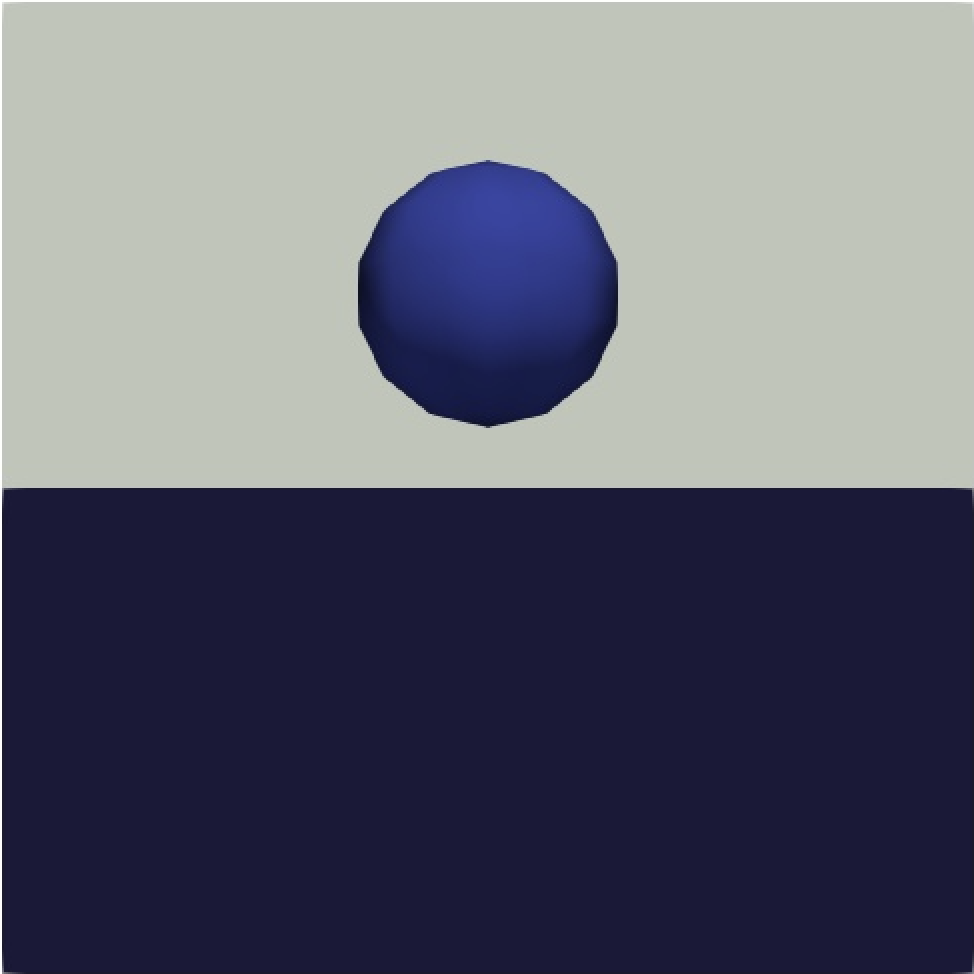
\includegraphics[width=\linewidth]{GWU_Thesis_Sarmakeeva/Images/chap4/water_sphere/sphere_in_water0.png}
        \subcaption{0.1 sec}
    \end{minipage}%
    \hspace{0.05\textwidth}
    \begin{minipage}{.4\textwidth}
        \centering
        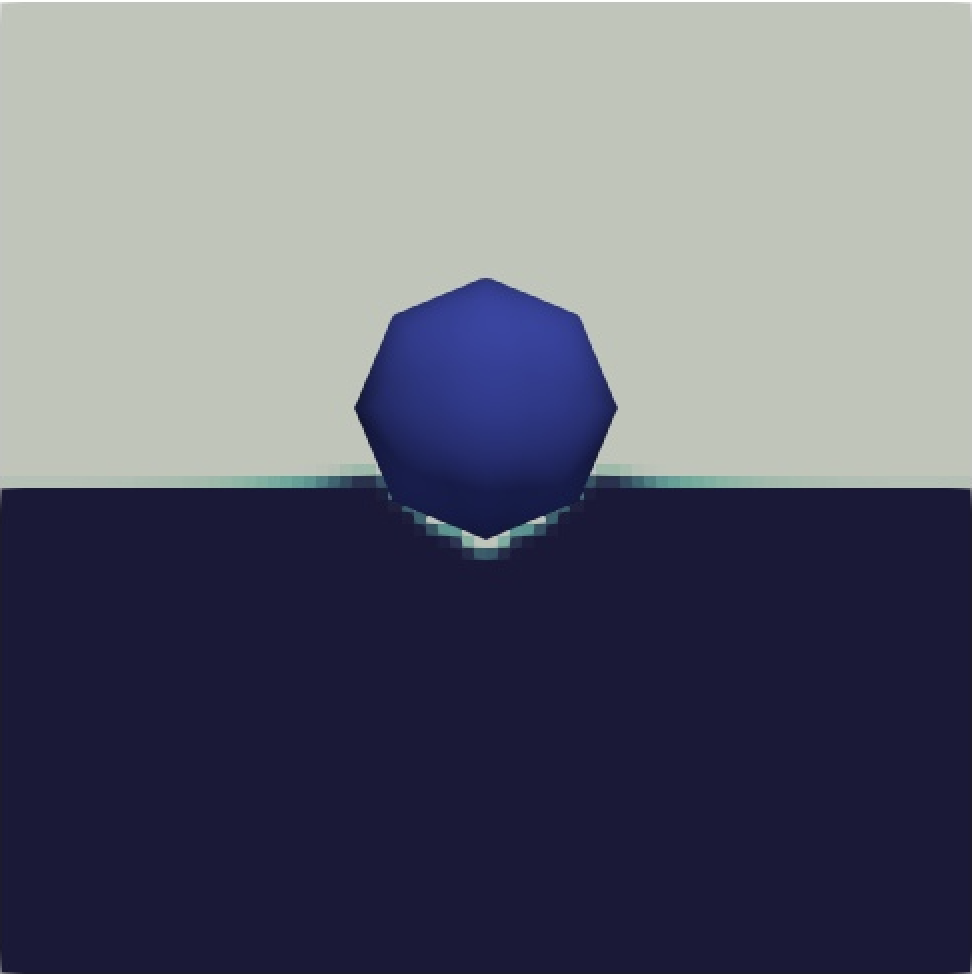
\includegraphics[width=\linewidth]{GWU_Thesis_Sarmakeeva/Images/chap4/water_sphere/sphere_in_water02.png}
        \subcaption{0.2 sec}
    \end{minipage}
    \newline
    \begin{minipage}{.4\textwidth}
        \centering
        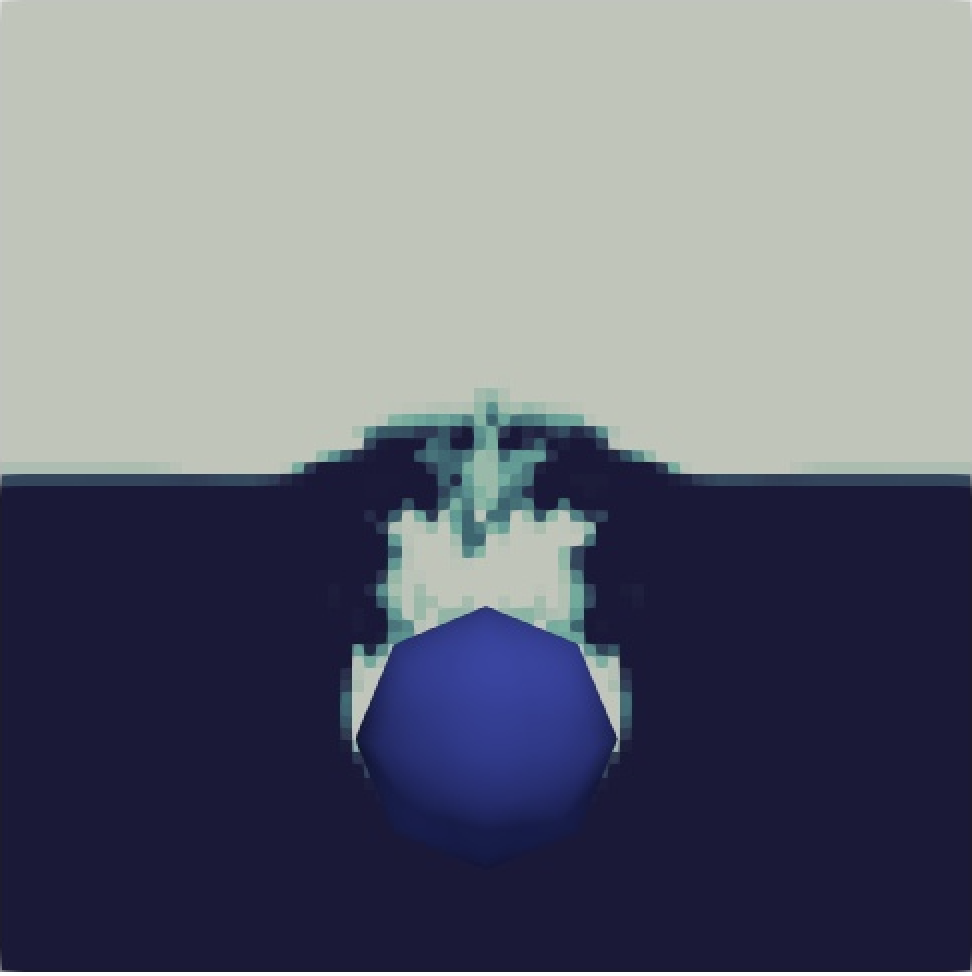
\includegraphics[width=\linewidth]{GWU_Thesis_Sarmakeeva/Images/chap4/water_sphere/sphere_in_water04.png}
        \subcaption{0.4 sec}
    \end{minipage}%
    \hspace{0.05\textwidth}
    \begin{minipage}{.4\textwidth}
        \centering
        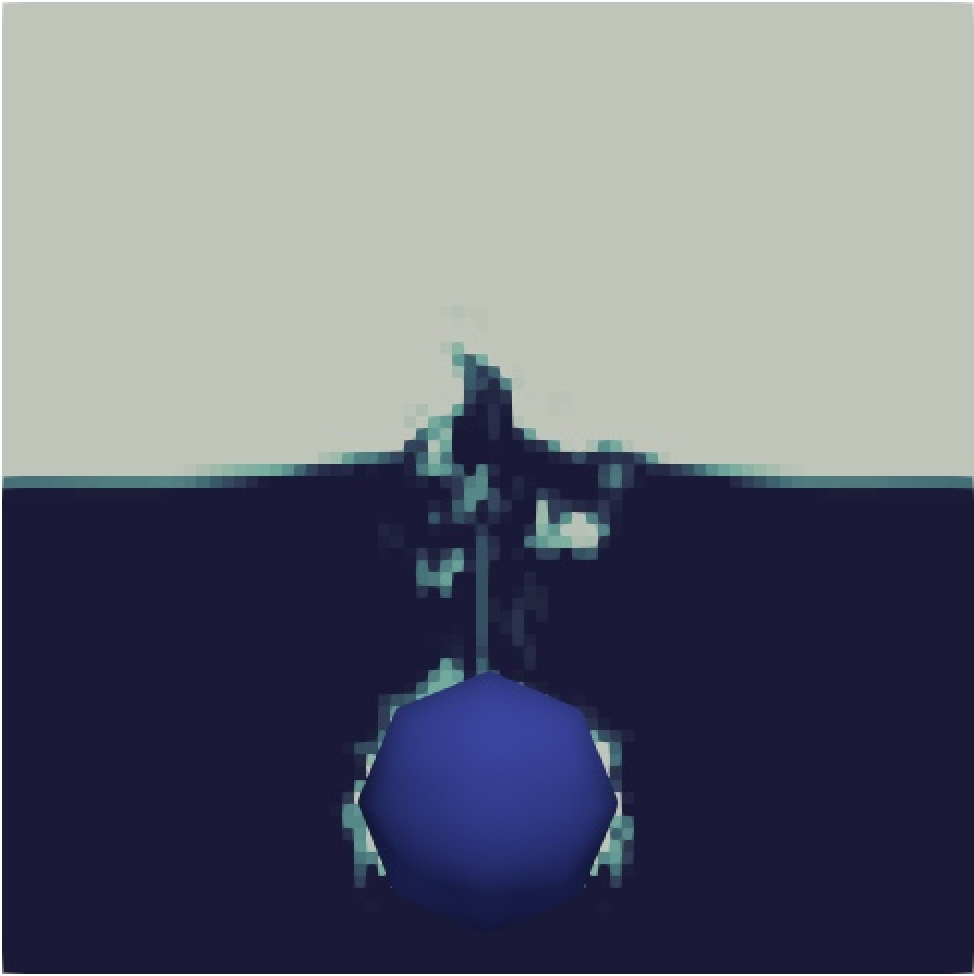
\includegraphics[width=\linewidth]{GWU_Thesis_Sarmakeeva/Images/chap4/water_sphere/sphere_in_water07.png}
        \subcaption{0.7 sec}
    \end{minipage}
    \newline
    \begin{minipage}{.4\textwidth}
        \centering
        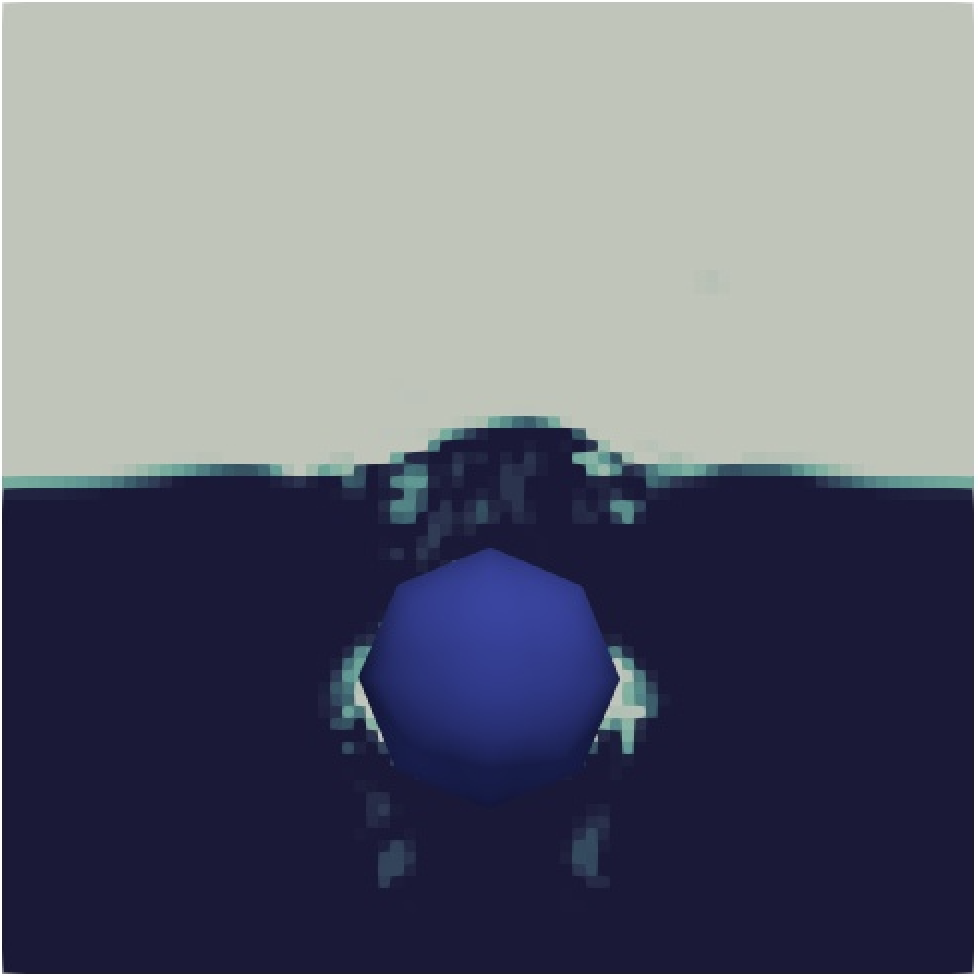
\includegraphics[width=\linewidth]{GWU_Thesis_Sarmakeeva/Images/chap4/water_sphere/sphere_in_water09.png}
        \subcaption{0.9 sec}
    \end{minipage}%
    \hspace{0.06\textwidth}
    \begin{minipage}{.4\textwidth}
        \centering
        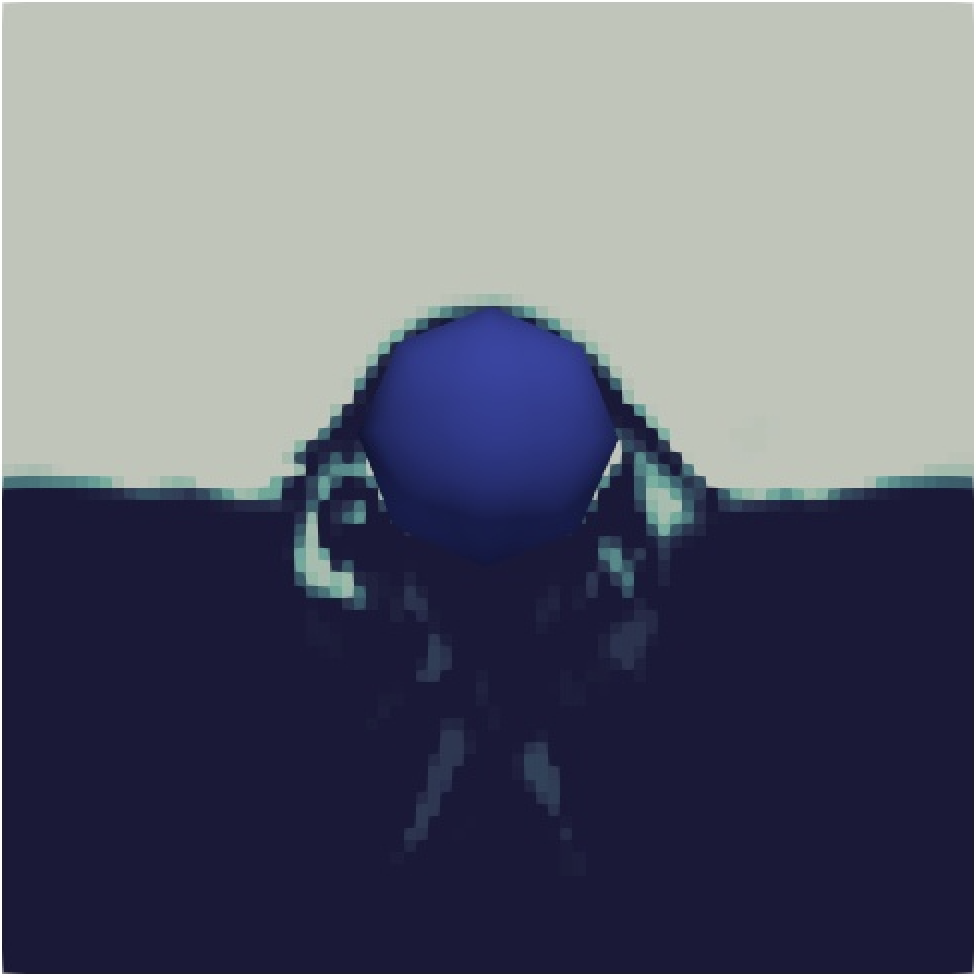
\includegraphics[width=\linewidth]{GWU_Thesis_Sarmakeeva/Images/chap4/water_sphere/sphere_in_water12.png}
        \subcaption{1.2 sec}
    \end{minipage}
    \caption{Visualization of sphere bouncing in two-phase fluid from CFD-DEM simulation.}
    \label{fig:two-phase_sphere}
\end{figure}



 \begin{figure}[!ht]
    \centering
    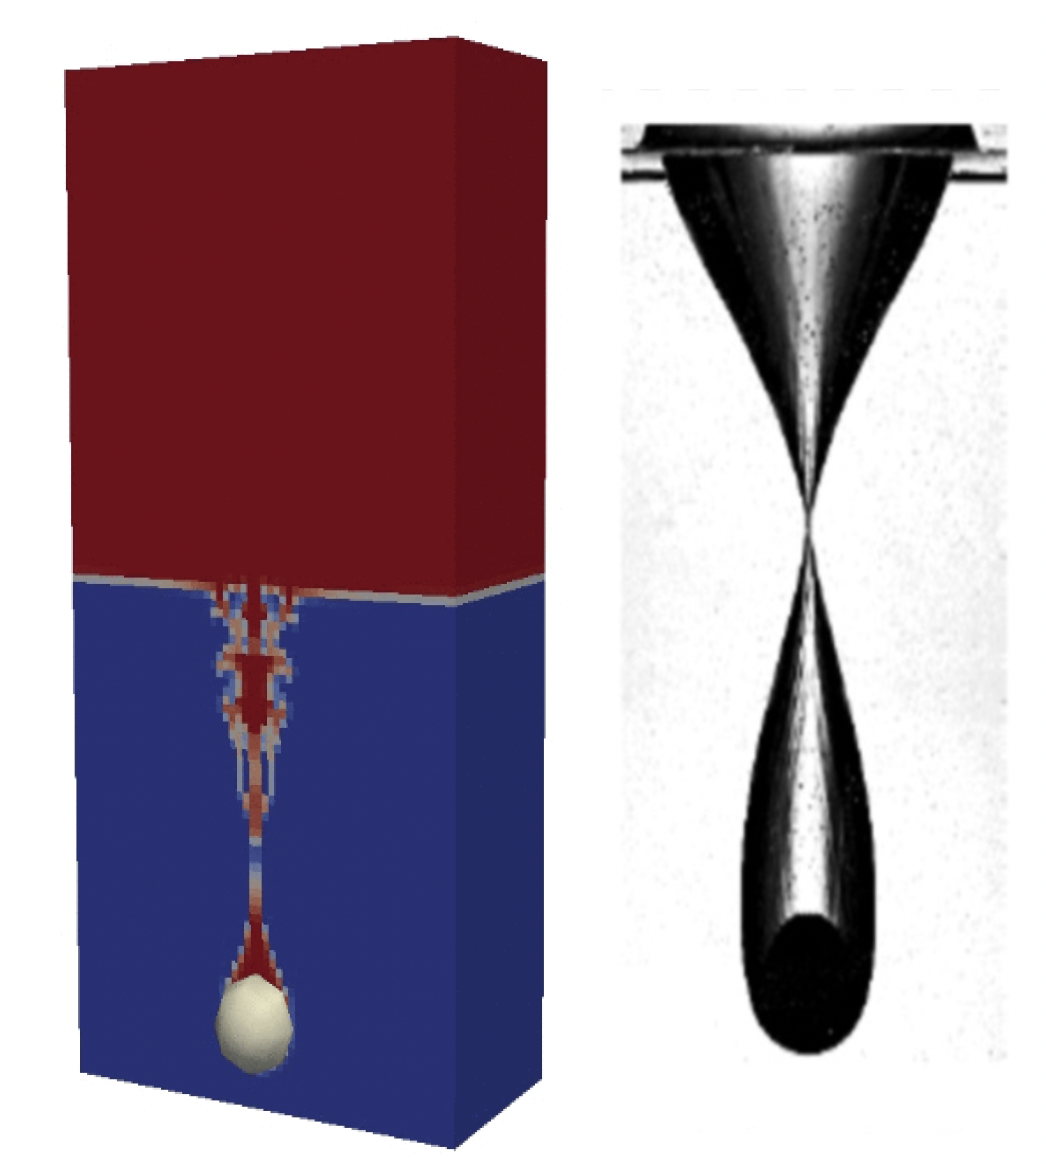
\includegraphics[width=12cm]{Images/chap3/cavityIB.png}
    \caption{Falling sphere visualization and comparison with the experiment \cite{schwalbach}. On the right, cavity after falling sphere in the water \cite{schwalbach}.}
    \label{fig:IB}
\end{figure}
Modeling the physical experiments involving a sphere falling into the water where the density of the sphere is more than the water, as outlined in Schwalbach et al. (2014) \cite{schwalbach}, was challenging. One primary obstacle is that the original paper did not to include the height from which the sphere is dropped. This parameter has a significant impact on the free surface during the simulation and is essential for ensuring that the solution will converge. Moreover, the movement of the free surface is dependent on the height at which the sphere being dropped. Despite this, the trajectory of the falling sphere in our simulations aligns well, the trace after the sphere penetrates the water and interacts with the free surface shows a similar fluid behaviour to the physical experiments, suggesting that our results are both stable, the solution converges, and comparable. Another study, \cite{shen2022resolved}, also attempts to replicate the original experiment through numerical methods. Again, this paper, in the same way, neglects to specify the height from which the spheres were dropped, making a complete comparison of results problematic.

\subsubsection{Computational setup}

For the numerical simulation of a sphere falling into water, we employ a two-phase flow model to capture the interaction between the solid sphere and the fluid phase. The Volume of Fluid (VOF) method is used to track the free surface between the air and water phases. Specifically, we incorporated the IsoAdvector \cite{roenby2019isoadvector} scheme, which is a robust and accurate approach for simulating complex free surface flows, as described in the Chapter \ref{chap:intro} and the Chapter \ref{chap:theory}

To solve the governing Navier-Stokes equations for the fluid flow, we apply the second-order Crank–Nicolson method for time differentiation. This method offers improved accuracy and stability compared to lower-order time integration schemes, which is crucial for capturing the transient flow dynamics associated with the falling sphere. The convection and diffusion terms in the Navier-Stokes equations are discretized using the \textit{Gausslinear} scheme, a second-order accurate finite volume method that interpolates the solution from cell centers to face centers using Gaussian integration.

The pressure field use tolerance of $10^{-6}$ and three PISO (Pressure Implicit with Splitting of Operators) loops per time step to ensure convergence. For the time step, we choose $\Delta t = 10^{-5}$ for the VOF calculations and $\Delta t = 10^{-6}$ for the Discrete Element Method (DEM) part. The DEM and VOF solvers communicate every ten time steps to solve the two-way coupling between the solid and fluid phases.

We carried out the simulations in a high-performance computing system. The key specifications of the system CPU are AMD Ryzen Threadripper PRO 3995WX, 64-Core, 128-Thread, with frequencies ranging from 2200 MHz to 4308.4 MHz. System Architecture: x86\_64, supporting 32-bit and 64-bit operations. Operating System: Linux-based.
\section{Multispherical body simulations}

\subsection{Multispherical body interaction with two-phase fluid}

The primary objective of this experiment is to illustrate the initial accuracy and functionality of the developed CFD-DEM code by simulating the interaction of a multi-spherical body, analogous to a previous experiment with a floating sphere in water Pathak et al.(2016) \cite{pathak20163d}.

The simulation involves a multi-spherical body consisting of 2 overlapping spheres positioned at a $0.4$ m height above a fluid with the properties of water. The main properties are provided in Table \ref{table3-chap4} below.
\begin{table}[H]
    \centering
    \caption{Simulation Parameters} \label{table3-chap4}
    \begin{tabular}{llr}
        \toprule
        \hline
        Simulation Part         & Physical Parameters (units) & Value \\
        \hline
        \midrule
        Particle 1                & Density (kg/m$^3$)          & 500    \\
                         & Diameter (m)          & 0.25    \\
                         & Initial height (m)          & (0.5, 0.5, 1.4 )  \\
        Particle 2                & Density (kg/m$^3$)          & 500    \\
                         & Diameter (m)          & 0.25   \\
                         & Initial height (m)          &  (0.2, 0.4, 1.4)     \\
                         \hline
                                 Fluid                  & Density (kg/m$^3$)           & $1000$   \\
                                & Viscosity (m$^2$/s)         & 1e$^{-6}$    \\
                                \hline
         Air                  & Density (kg/m$^3$)           & $1e-5$   \\
                                & Viscosity (m$^2$/s)         & 1e$^{-6}$    \\
                                \hline
        \bottomrule
     \end{tabular}
\end{table}

The body is released and allowed to fall into the water under gravity forces. The simulation captures the motion of the body and the fluid's response upon impact and during the subsequent settling period. The results of the simulation are shown in figure \ref{fig:two-phase exp} below.

\begin{figure}[!ht]
  \centering
  \begin{tabular}{cc}
    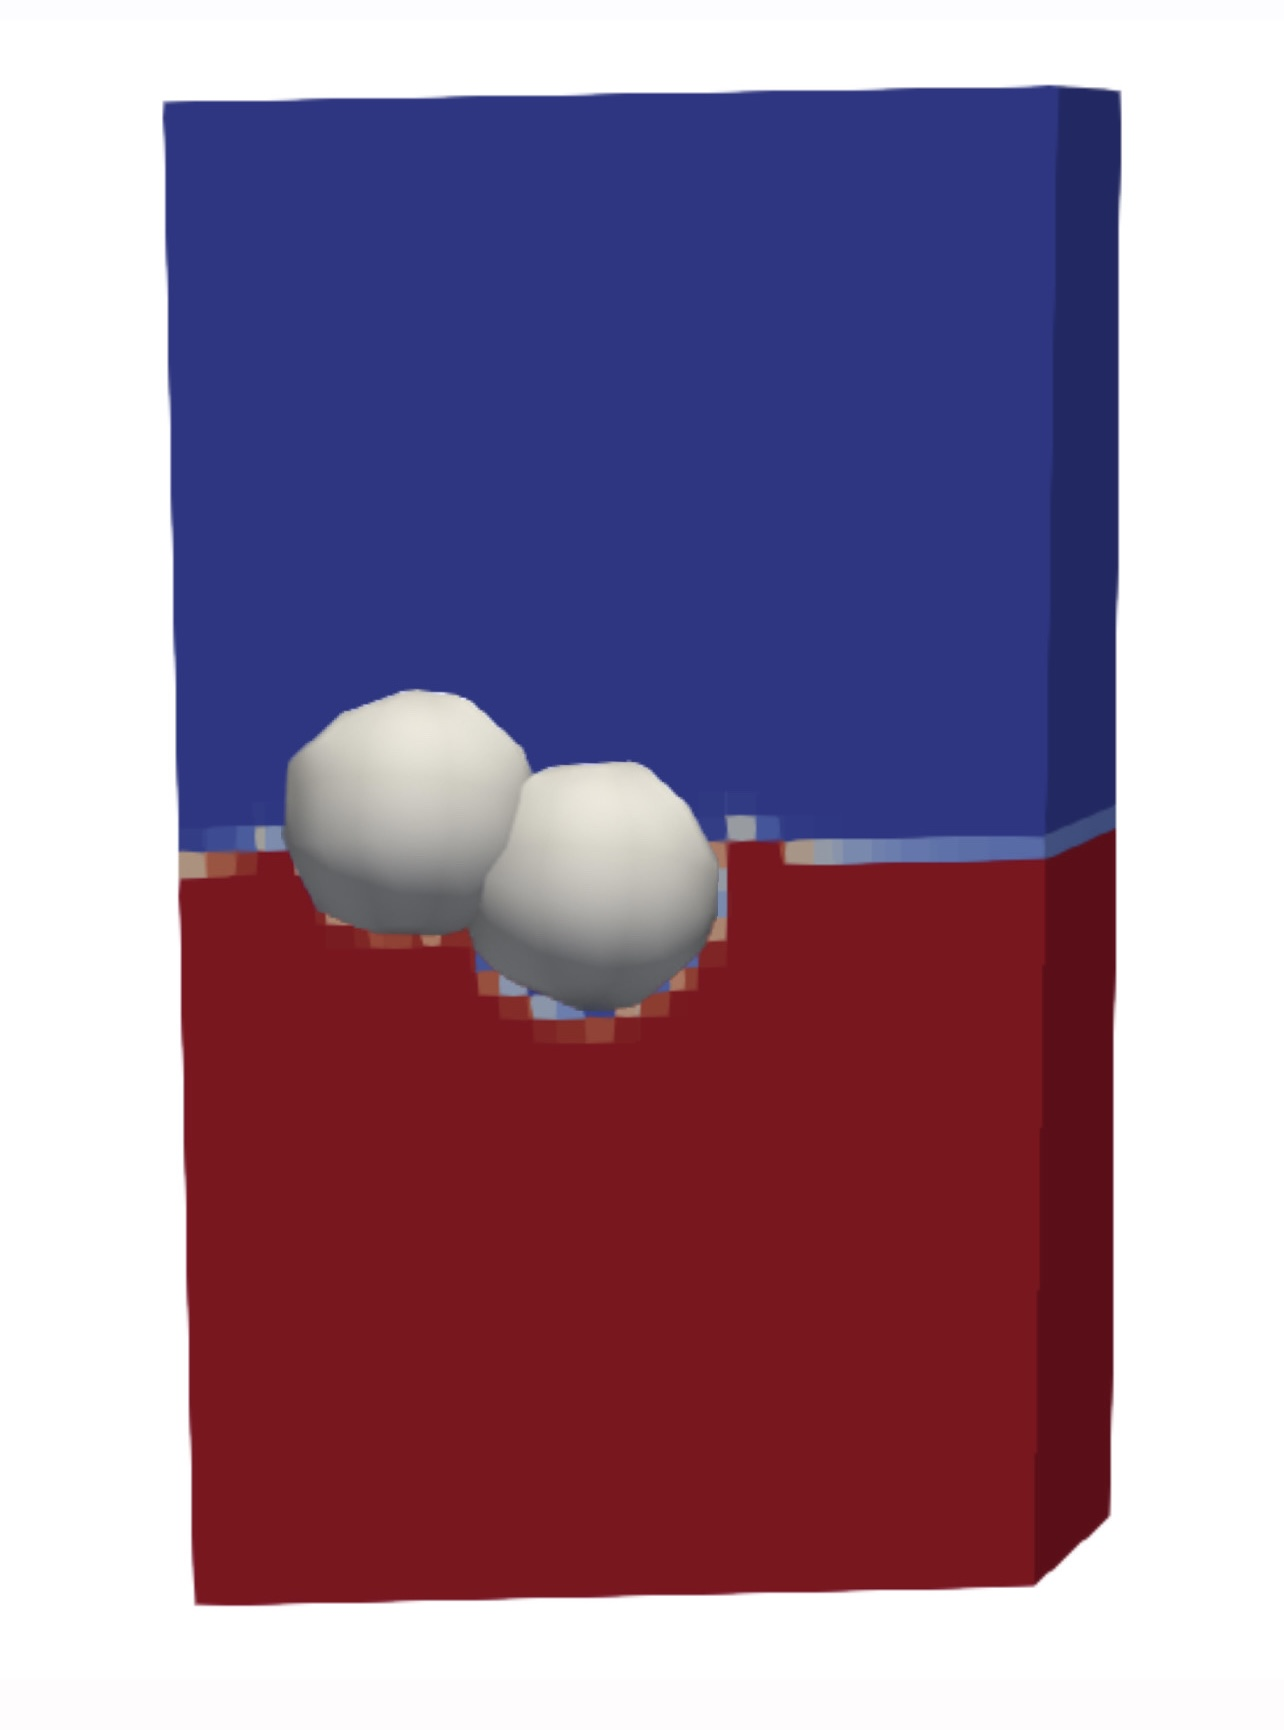
\includegraphics[width=0.4\textwidth]{Images/chap3/2_sph_2.jpg} & 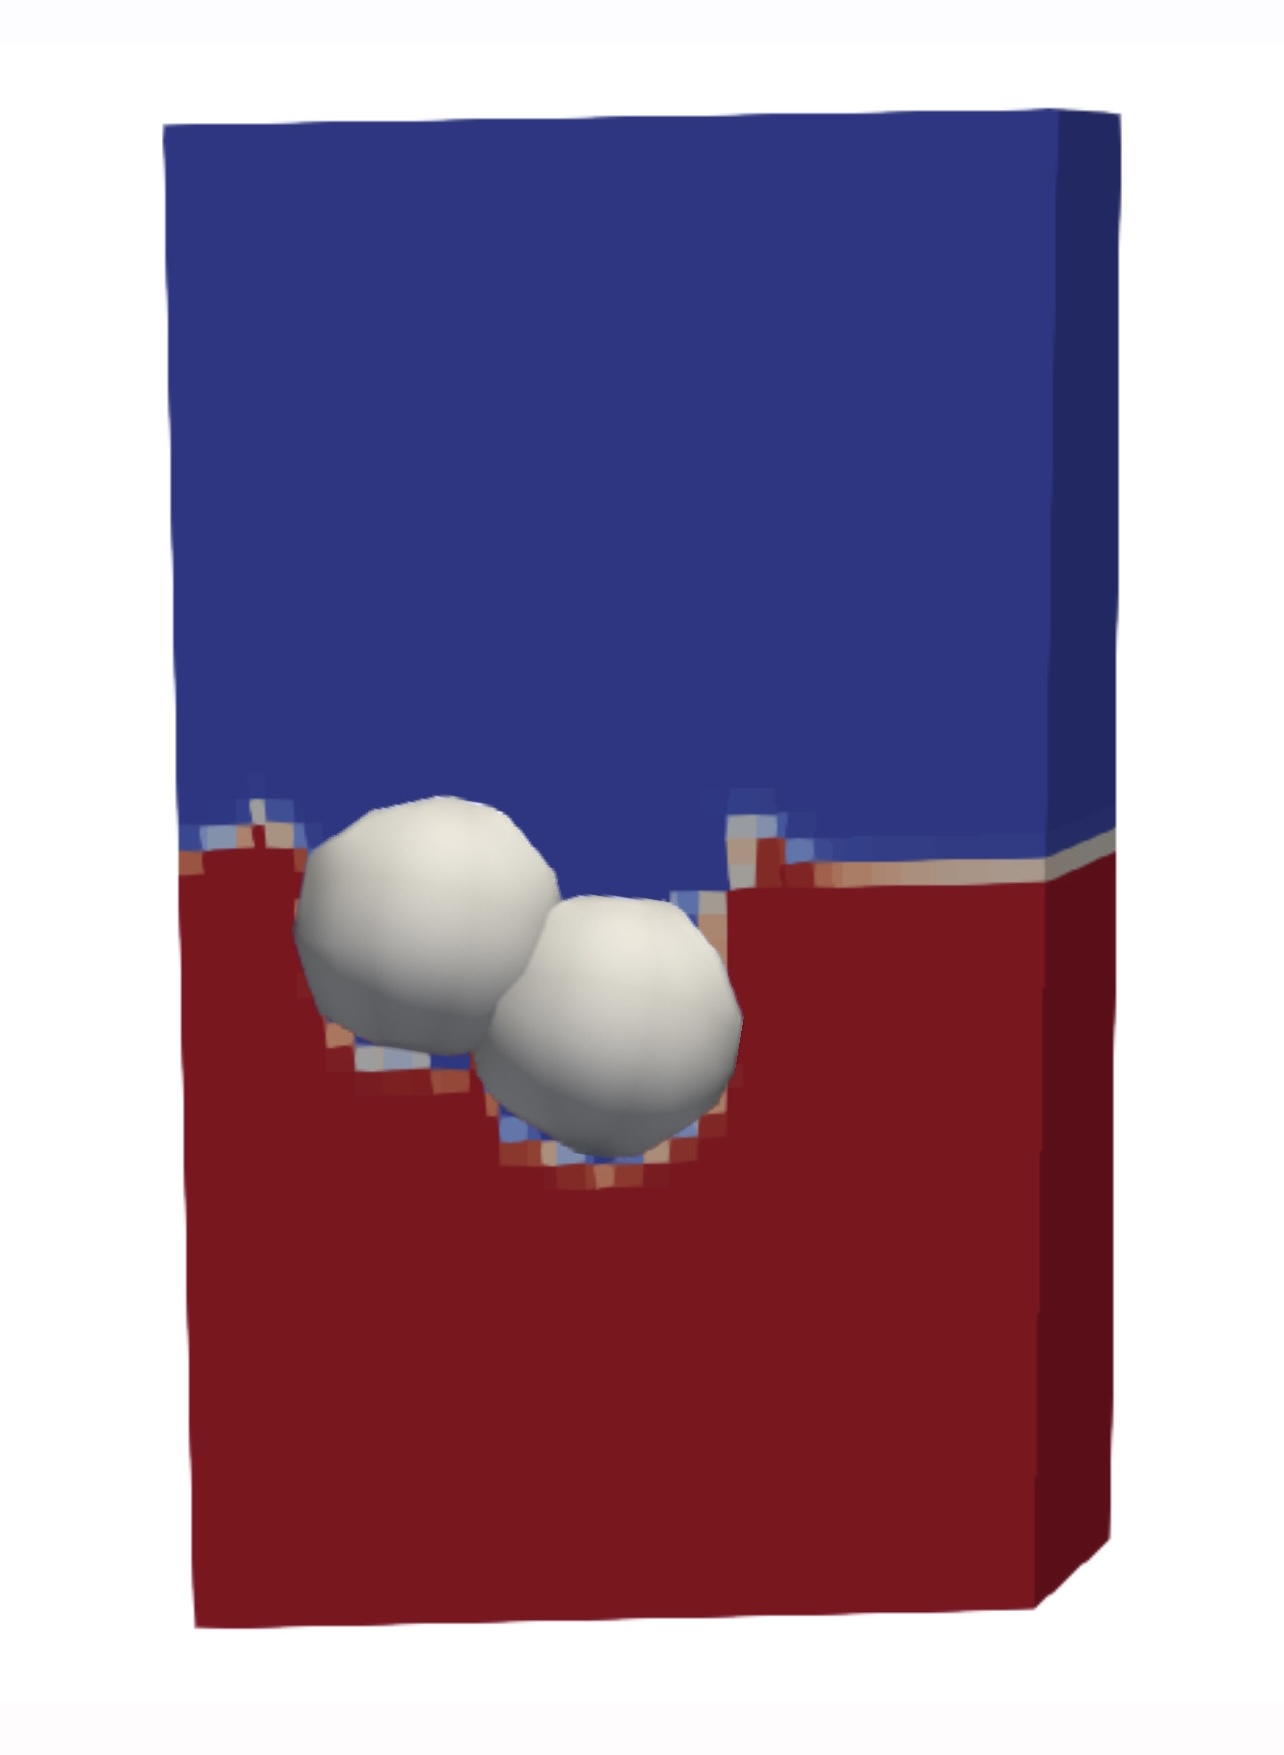
\includegraphics[width=0.4\textwidth]{Images/chap3/2_sph_1.jpg} 
    %(a) 0. s & (b) 0.35 s \\
  \end{tabular}
  \caption{Multispherical body created out of two spheres bouncing in liquid.}
  \label{fig:two-phase exp}
\end{figure}

The results of the simulation showed the numerical stability of the solver. When the fluid undergoes significant changes and spheres fall into the water, the presented numerical scheme converges. This was a significant challenge while we were running the simulation. This is why testing bouncing multispherical bodies interacting with a free surface was an important part of the research. Another concern was the volume of fluid phases; it changes in the range less than 1\%.

\subsection{Multispherical sinking body simulations}

A couple of works use similar approaches recently published for landslide simulations as Nan et al. (2023) \cite{nan2023high} and Shen et al. (2022) \cite{shen2022resolved}.
Like them, we run the simulations with one multi-spherical body falling into the water and multiple arbitrarily shaped bodies falling under gravity force, interacting with each other and interacting with water.


\begin{figure}[H]
    \centering
    \begin{minipage}{.5\textwidth}
        \centering
        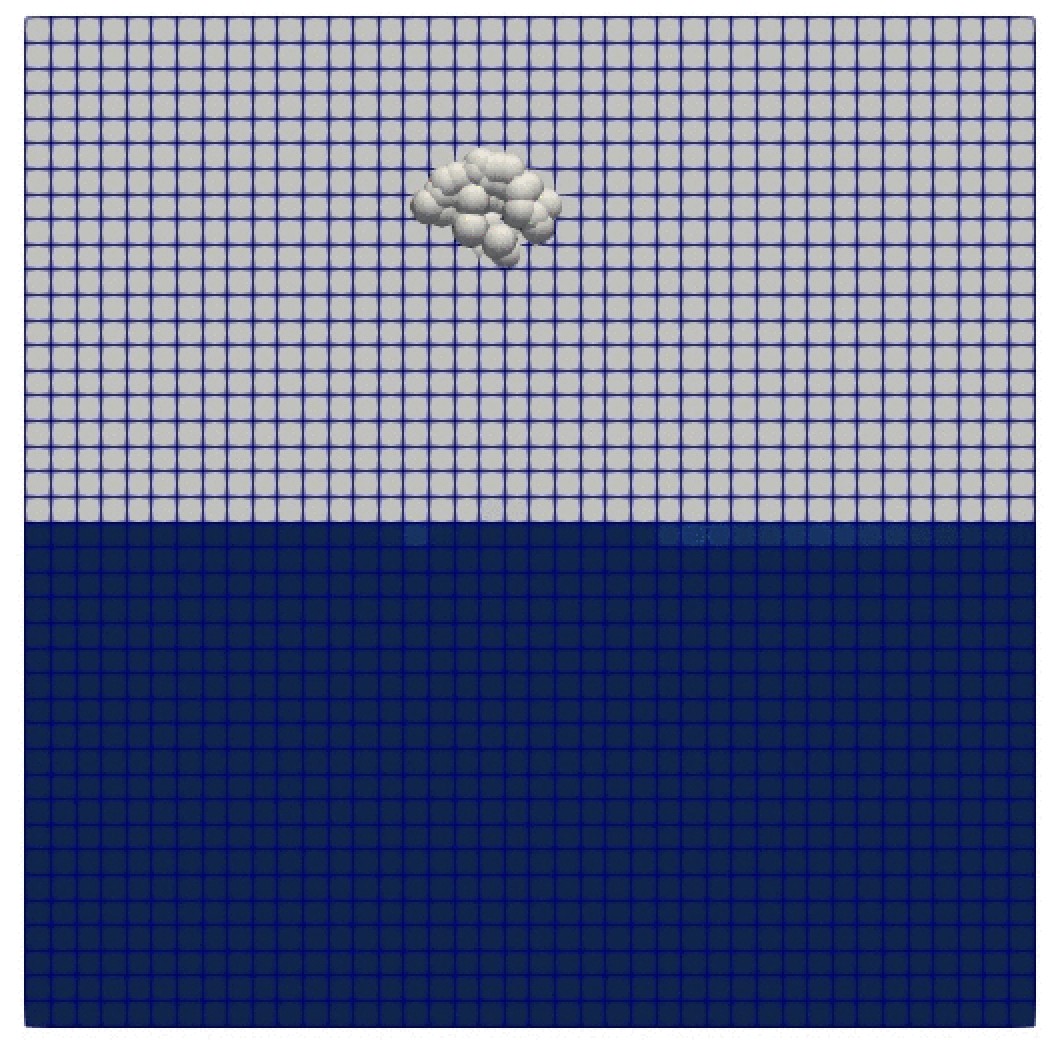
\includegraphics[width=\linewidth]{GWU_Thesis_Sarmakeeva/Images/chap4/clump_1.png}
        \subcaption{0 sec}
        %(a) 0. s
    \end{minipage}%
    \begin{minipage}{.5\textwidth}
        \centering
        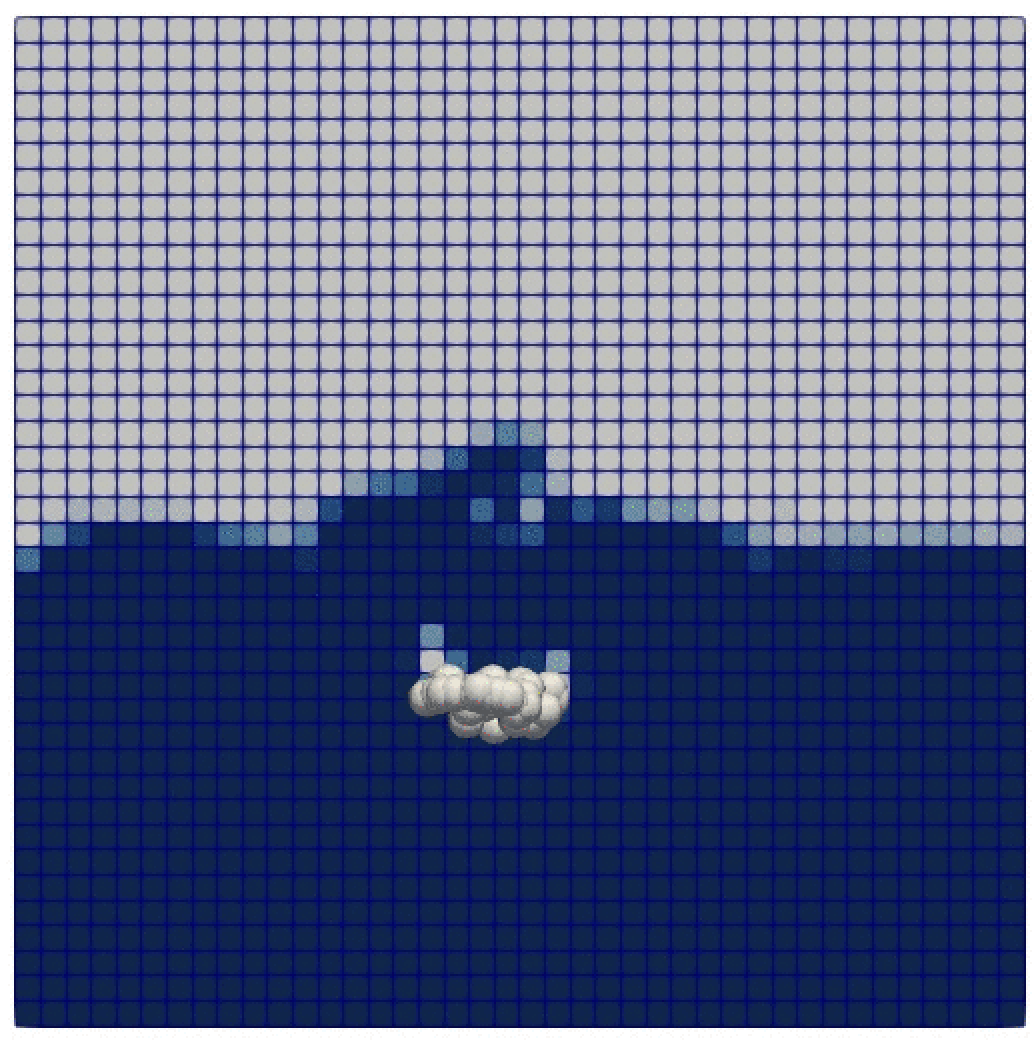
\includegraphics[width=\linewidth]{GWU_Thesis_Sarmakeeva/Images/chap4/clump_2.png}
        \subcaption{0.1 sec}
        %(b) 0.35 s
    \end{minipage}
    \newline
    \begin{minipage}{.5\textwidth}
        \centering
        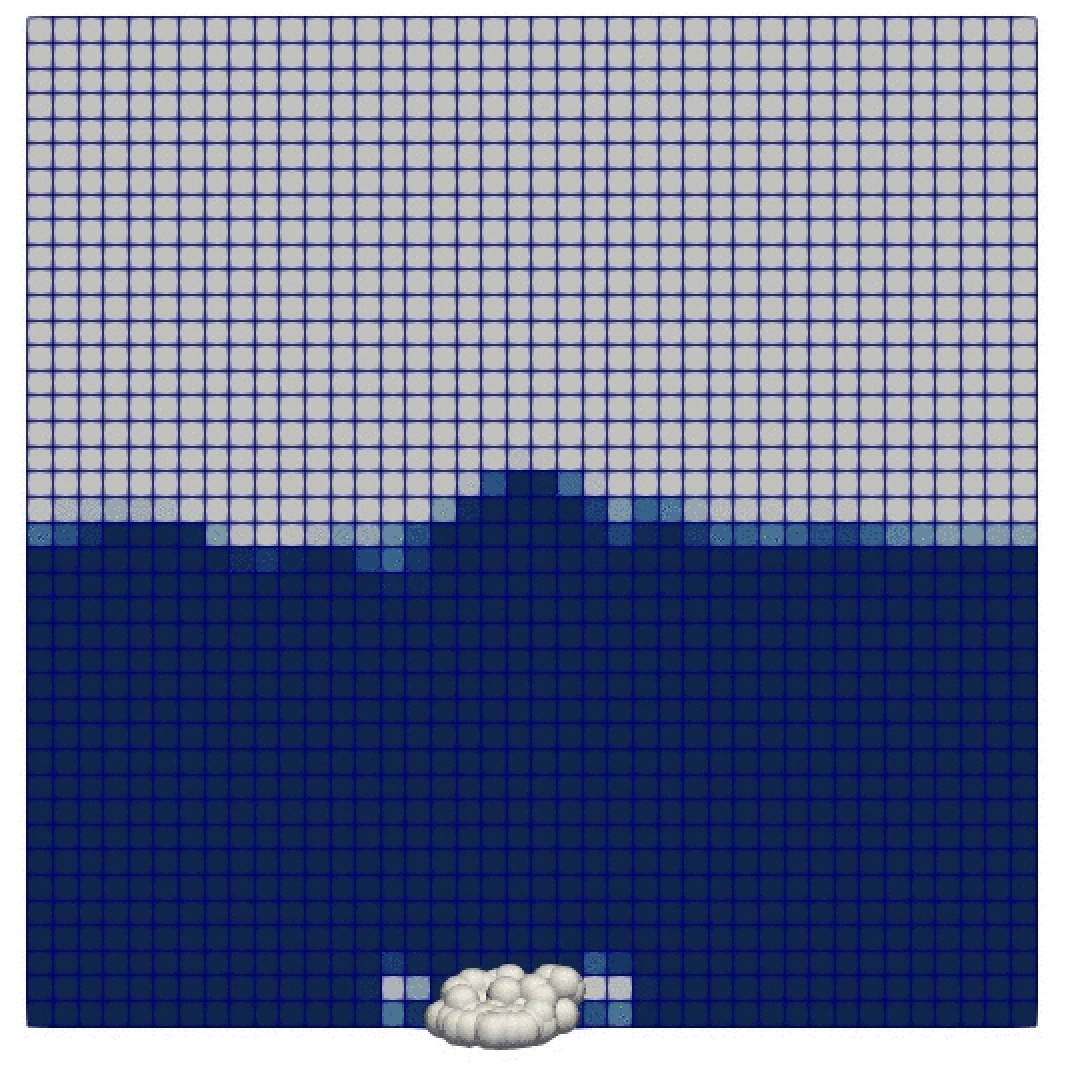
\includegraphics[width=\linewidth]{GWU_Thesis_Sarmakeeva/Images/chap4/clump_3.png}
        \subcaption{0.2 sec}
        %(c) Description
    \end{minipage}%
    \begin{minipage}{.5\textwidth}
        \centering
        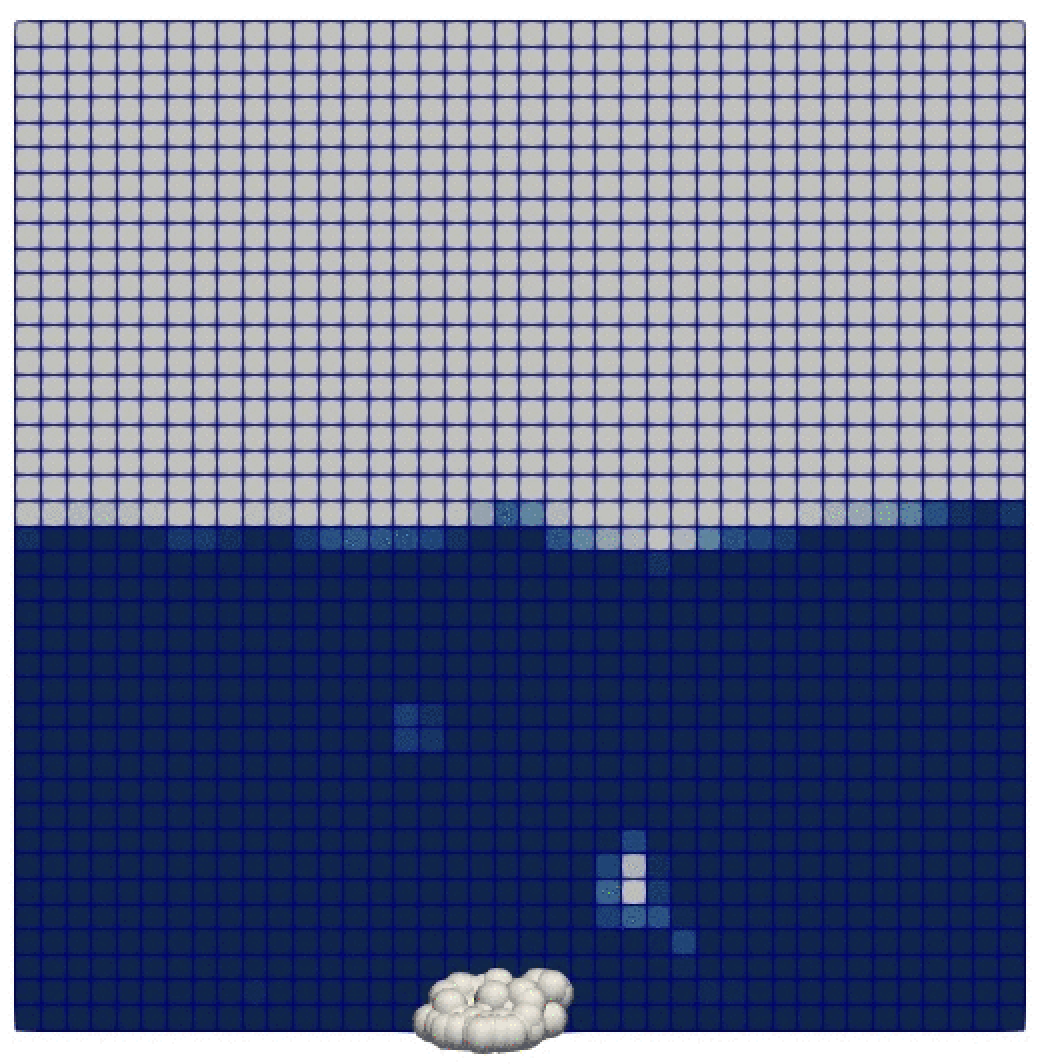
\includegraphics[width=\linewidth]{GWU_Thesis_Sarmakeeva/Images/chap4/clump_4.png}
        \subcaption{0.3 sec}
        %(d) Description
    \end{minipage}
    \caption{Falling multispherical body consisting of $n = 50$ spheres where a) initial clump placement b) after penetration into fluid c) body settled at the bottom of the container at 0.2 sec d) body settled at the bottom of the container at 0.3 sec.}
    \label{fig:two-phase_exp}
\end{figure}

First, we consider the falling clump - multispherical body experiment \ref{fig:two-phase_exp}. The solid body is made out of $50$ intersecting spheres with a density of 2500 kg/m$^3$ and set up in the area $x: 0.15 $ to $0.22$, $y: 0.1$ to $0.125$, $z: 0.3$ to $0.35$. The CFD domain is $0.4\times 0.3\times0.4$. The fluid level is on $y = 0.2$. The simulation ran for $0.3$s with $\Delta t = 5e-5$. The body falls under gravity force in the $z$-direction. 

Figure \ref{fig:two-phase_exp} captures the dynamic interaction between the multispherical body and the fluid, including the entry, sinking, and settling phases. The snapshots highlight the complexity of movement and deformation of a clump. Figure\ref{fig:two-phase exp}(a) shows the initial multispherical body placement, which is located between $0.3$ and $0.35$, the body starts to fall under the gravity force. In the second image \ref{fig:two-phase_exp} (b), we can see the body after penetration into the water. In figures \ref{fig:two-phase_exp} (c) and (d), we can see the body settled at the bottom of the container, and the fluid's free surface is stabilized.

The simulation result shows convergence of the numerical scheme for the resolved CFD-DEM method as well as during fluctuations of free surface and calculation of surface tension. Due to successful multispherical body interaction with fluid, for the next simulation, we increased the number of clumps but reduced the number of spheres in clumps. 



For multiple clumps (Figure \ref{fig:two-phase_exp_clumps}), the experiment includes 22 clumps made out of 18 spheres, in total 396 spheres falling under gravity force and interacting with the splashed water. The CFD area has 216000 computational cells, and the dimension of the domain is $0.4\times 0.3\times0.4$. The area filled with clumps is $x:0.2$ to $0.4$, $y: 0.0$ to $ 0.2$,$ z:0.0$ to $ 0.3$. The simulation ran for $0.3$s with $\Delta t = 5e-5$. The clumps fall under gravity force in $z$-direction.

Figure \ref{fig:two-phase_exp_clumps} (a) shows clumps placement at $0.05$ sec; the water column begins to collapse under gravity. Some clumps are submerged, while others are still in contact with the air. In the second Figure \ref{fig:two-phase_exp_clumps} (b), the body of water is almost entirely covered with clumps and moving in the $z$ direction under the gravity force. In Figures \ref{fig:two-phase_exp_clumps} (c) - (f), the column of fluid has collapsed further. We can see a splash of water hit the right boundary of the box and the bodies rotating and settling at the bottom of the container. The interaction between the fluid and the spherical bodies continues to evolve, and the flow continues to develop.

\newpage
\begin{figure}[H]
    \centering
    \begin{minipage}{.4\textwidth}
        \centering
        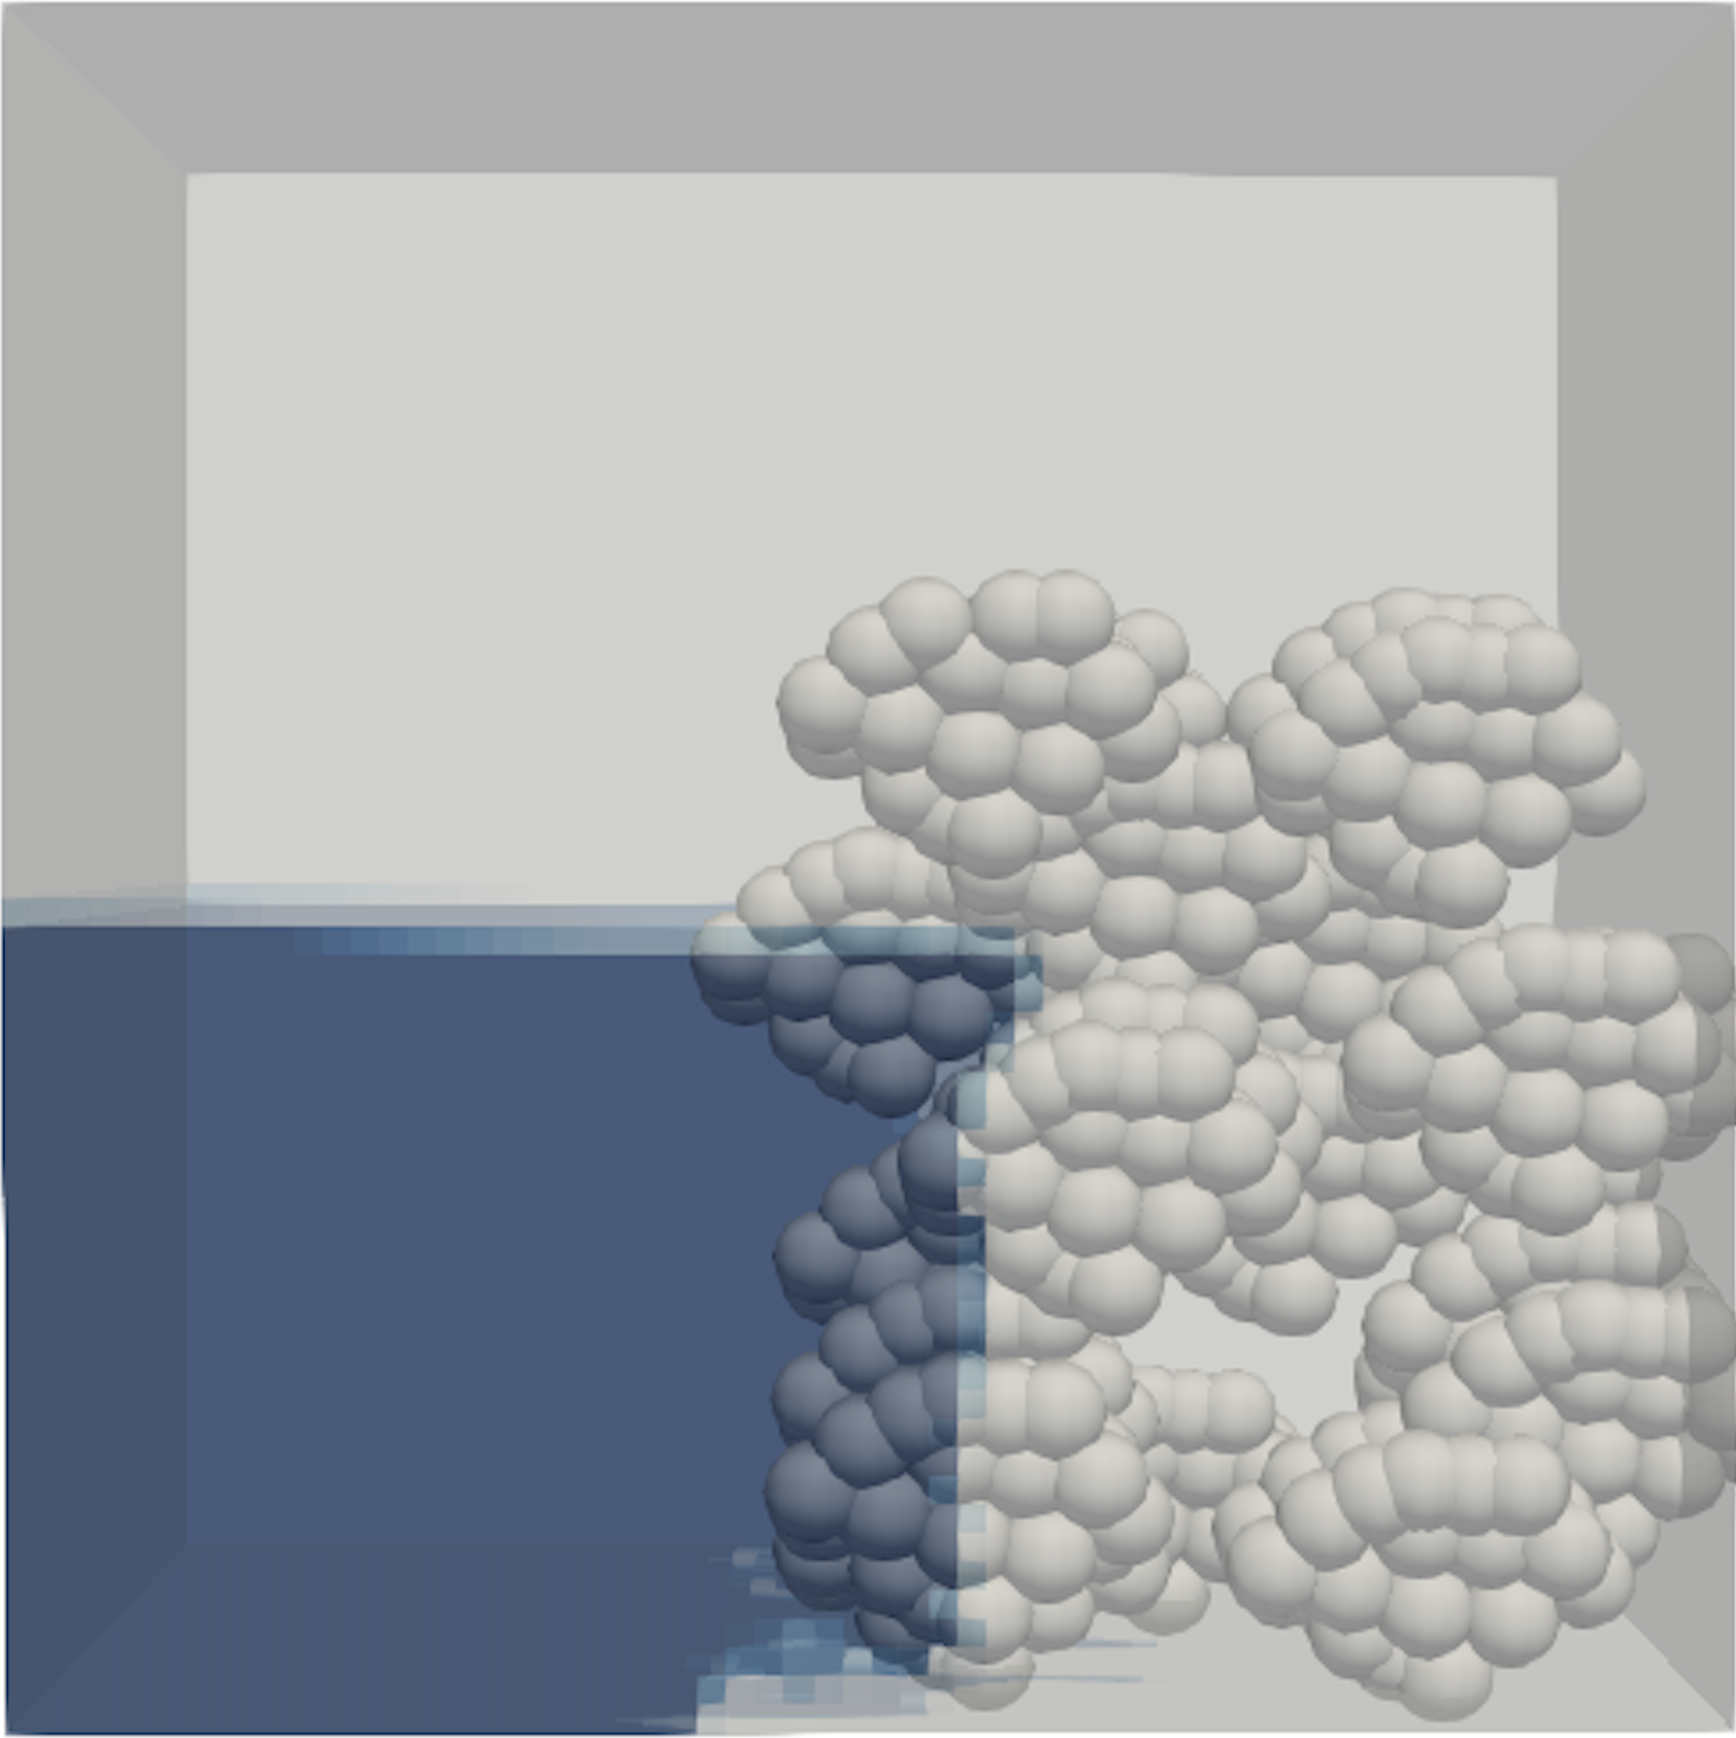
\includegraphics[width=\linewidth]{GWU_Thesis_Sarmakeeva/Images/chap4/landslide_1.png}
        \subcaption{0.05 sec}
    \end{minipage}%
    \hspace{0.05\textwidth}
    \begin{minipage}{.4\textwidth}
        \centering
        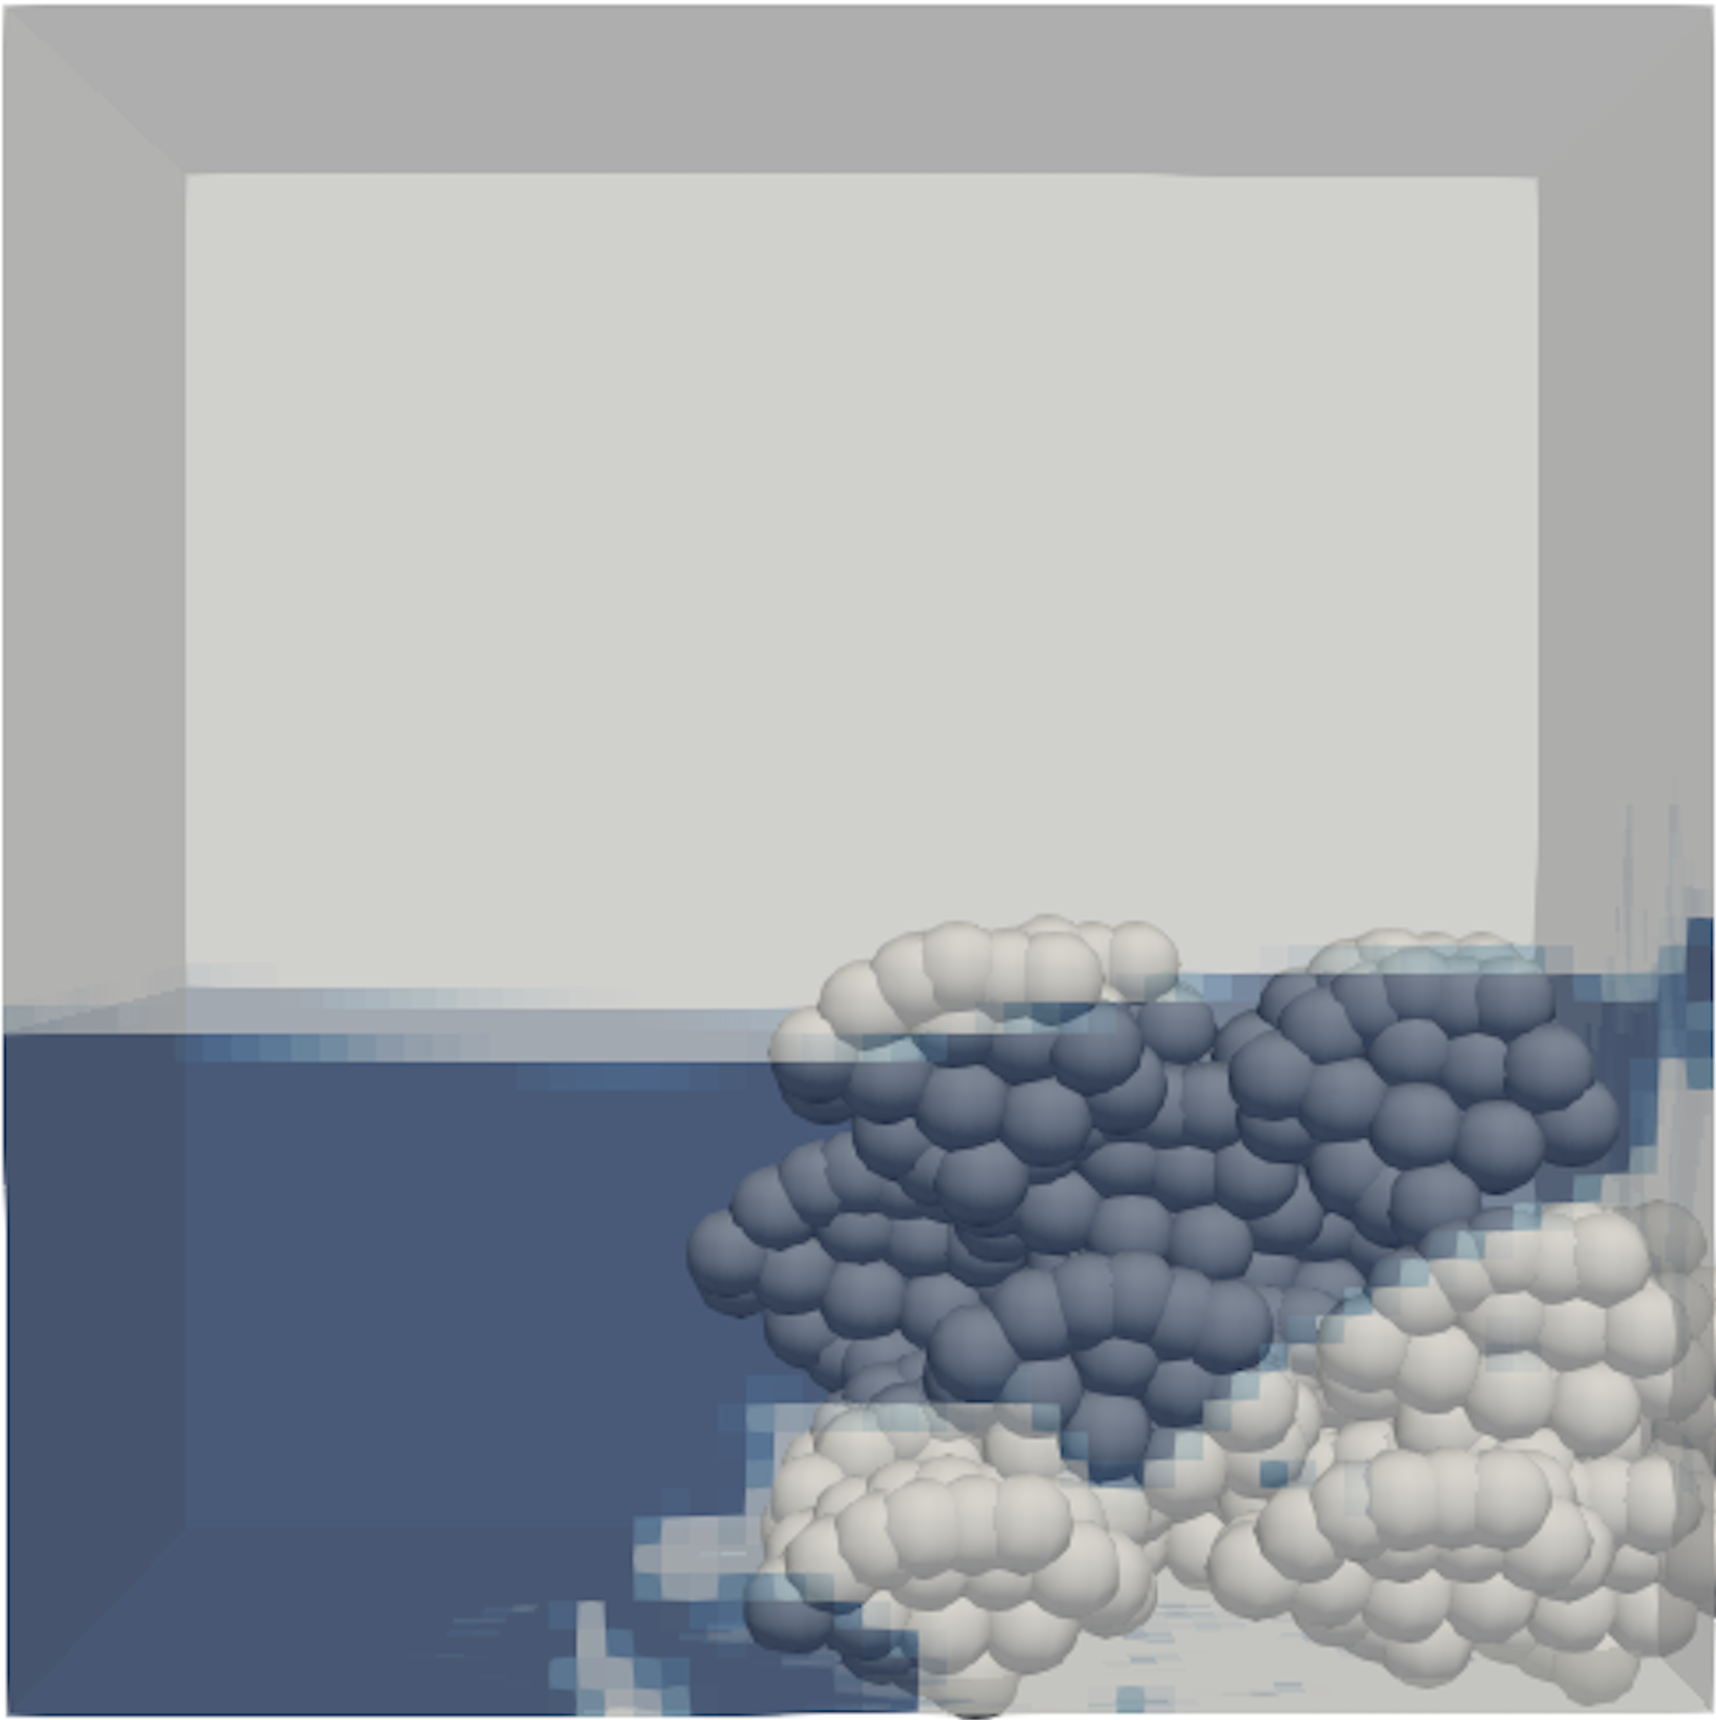
\includegraphics[width=\linewidth]{GWU_Thesis_Sarmakeeva/Images/chap4/landslide_2.png}
        \subcaption{0.1 sec}
    \end{minipage}
    \newline
    \begin{minipage}{.4\textwidth}
        \centering
        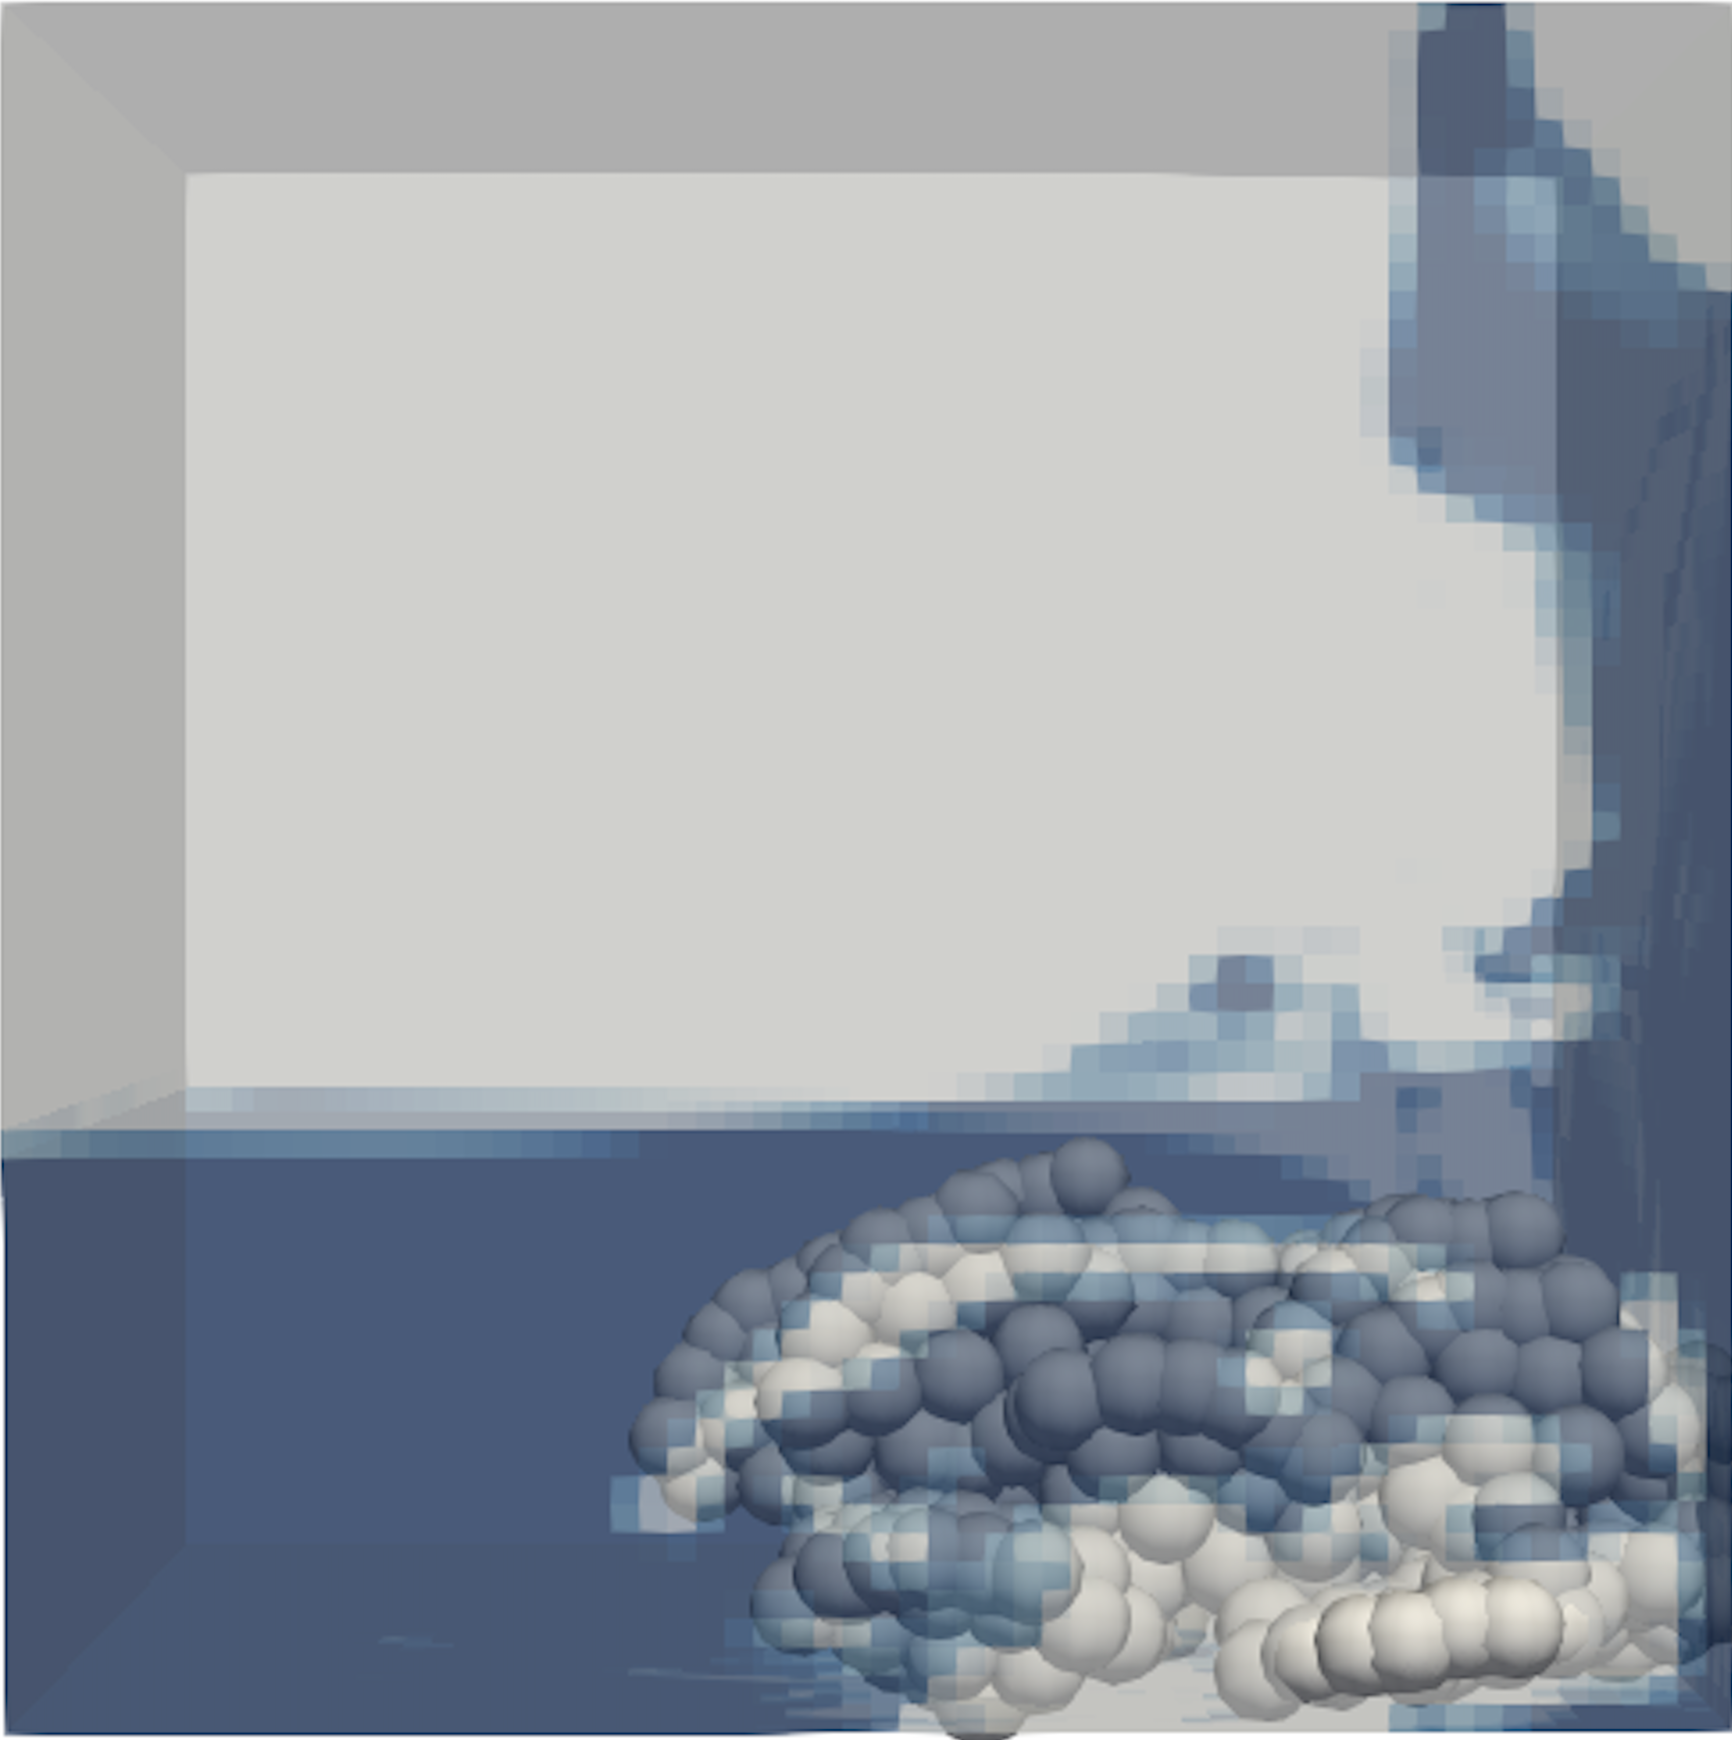
\includegraphics[width=\linewidth]{GWU_Thesis_Sarmakeeva/Images/chap4/landslide_3.png}
        \subcaption{0.15 sec}
    \end{minipage}%
    \hspace{0.05\textwidth}
    \begin{minipage}{.4\textwidth}
        \centering
        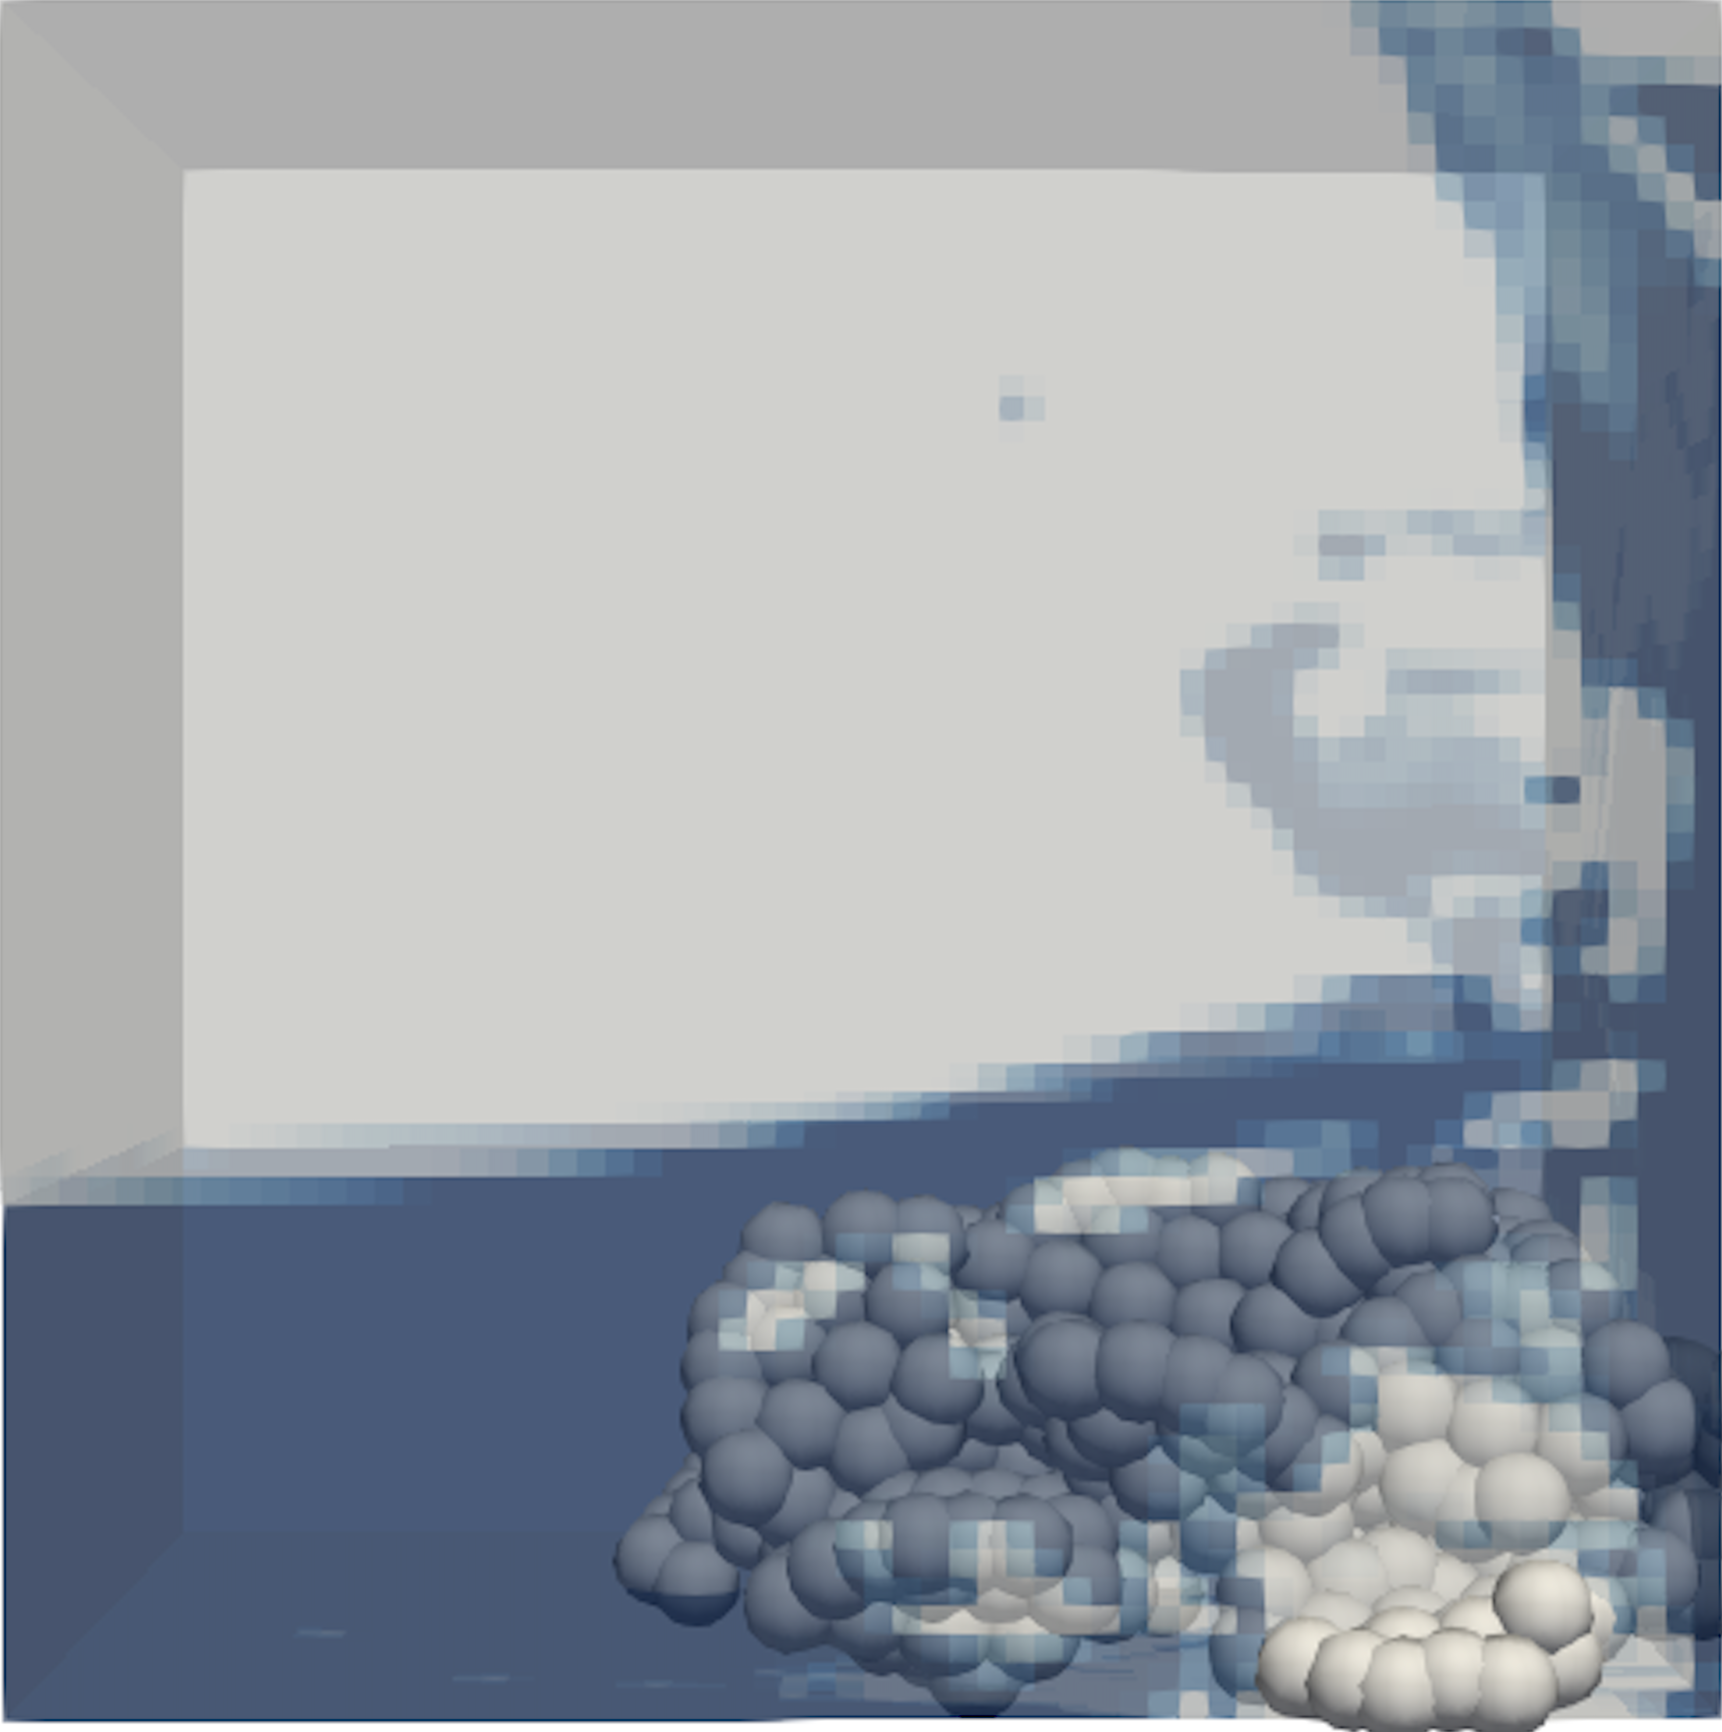
\includegraphics[width=\linewidth]{GWU_Thesis_Sarmakeeva/Images/chap4/landslide_4.png}
        \subcaption{0.2 sec}
    \end{minipage}
    \newline
    \begin{minipage}{.4\textwidth}
        \centering
        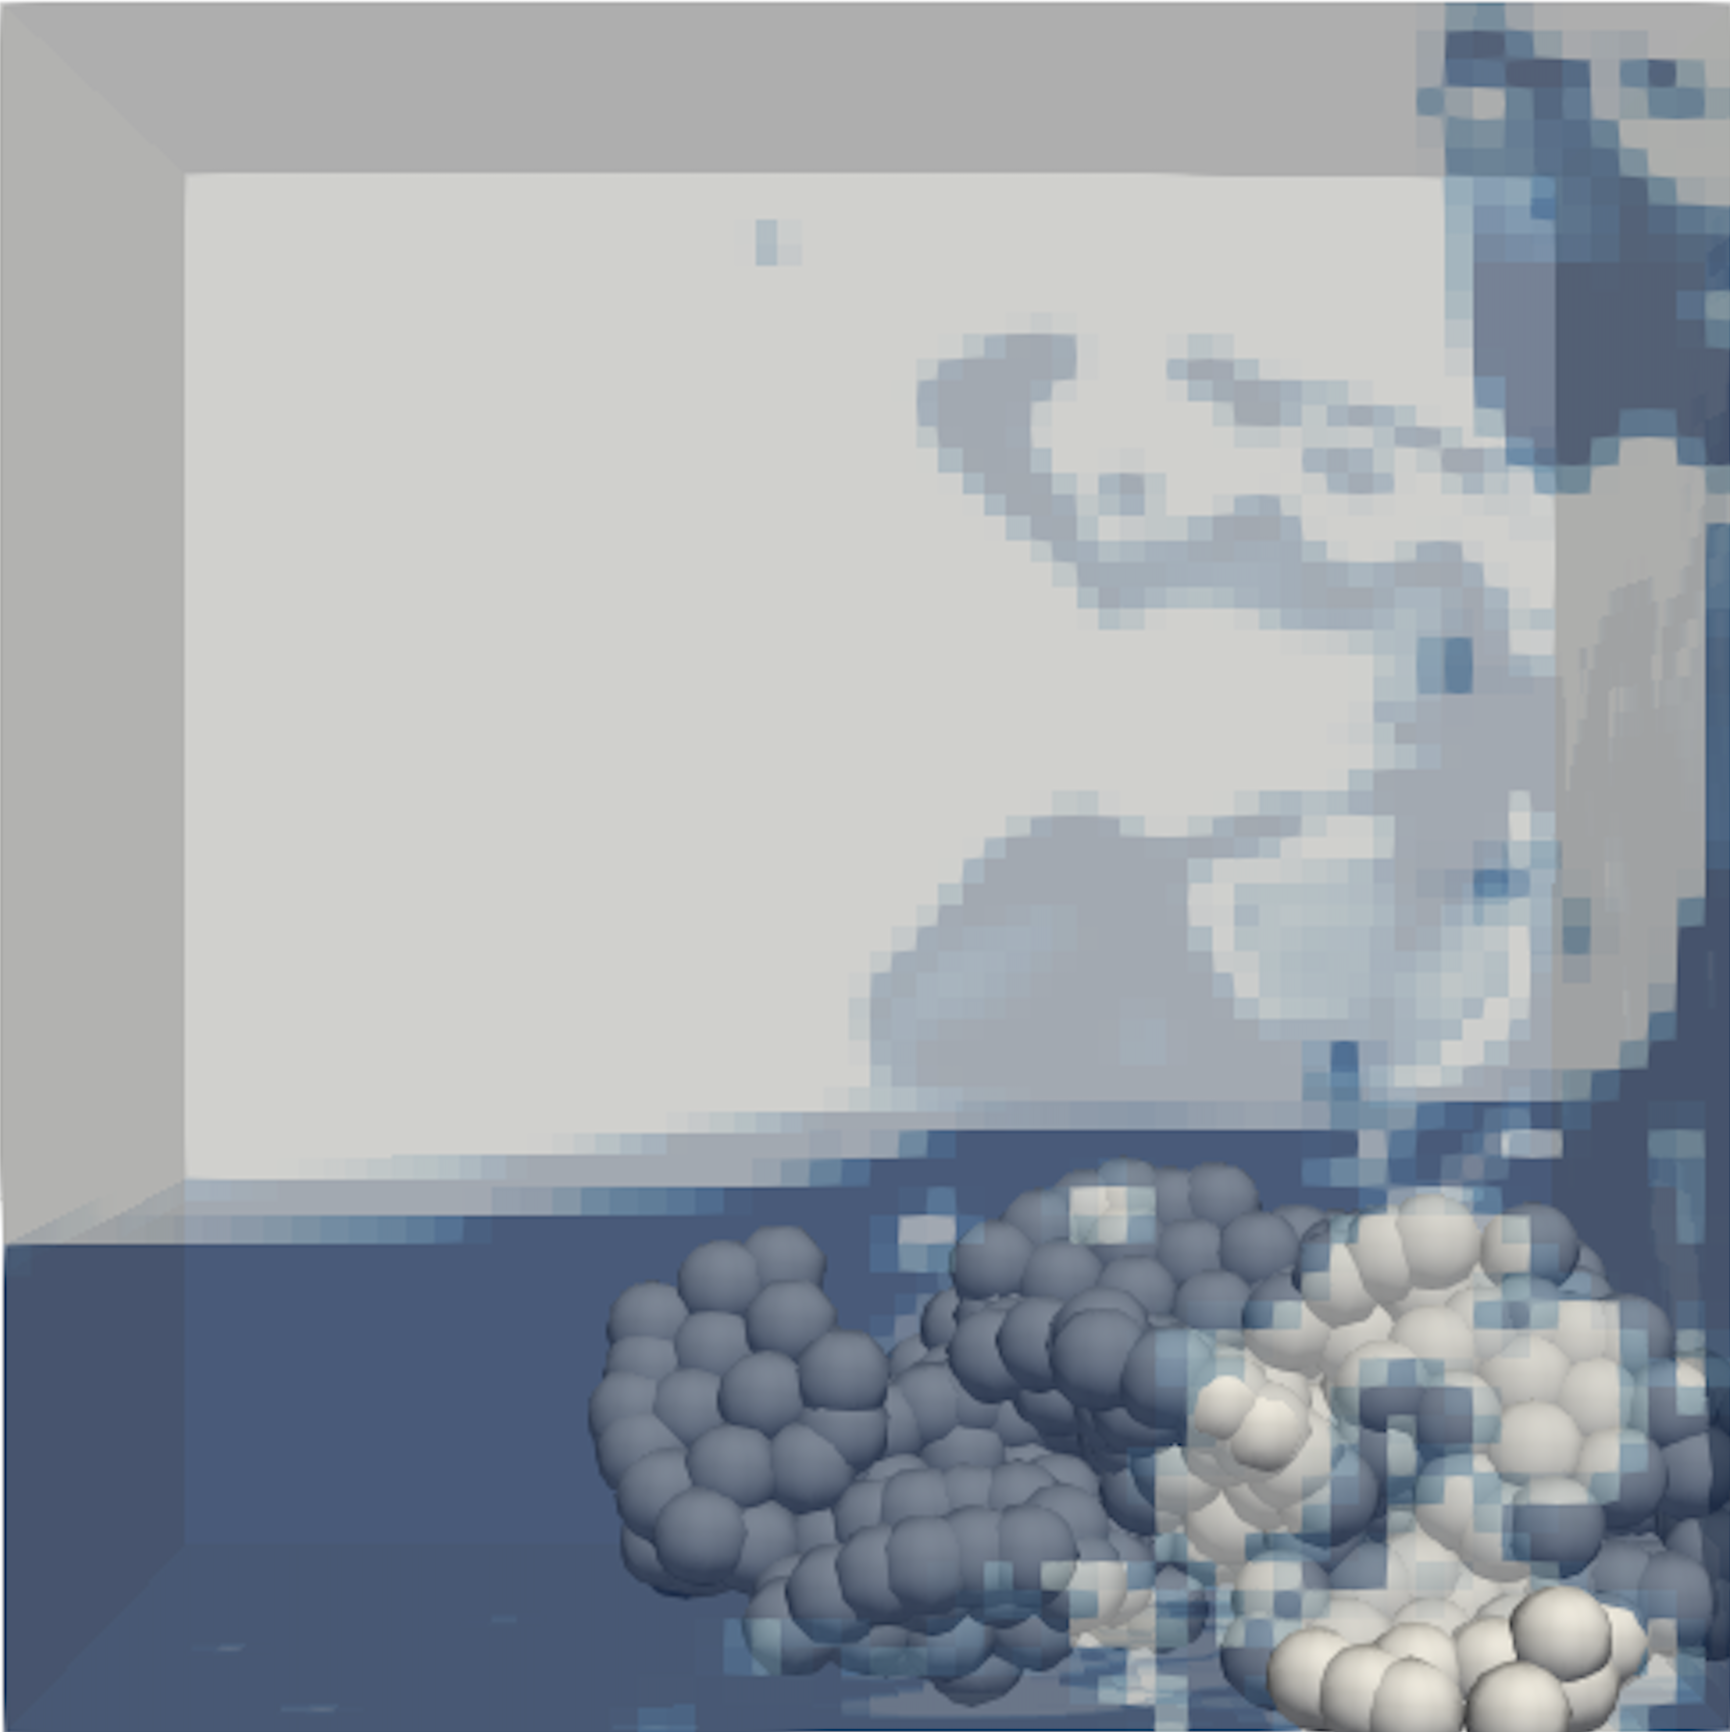
\includegraphics[width=\linewidth]{GWU_Thesis_Sarmakeeva/Images/chap4/landslide_5.png}
        \subcaption{0.25 sec}
    \end{minipage}%
    \hspace{0.06\textwidth}
    \begin{minipage}{.4\textwidth}
        \centering
        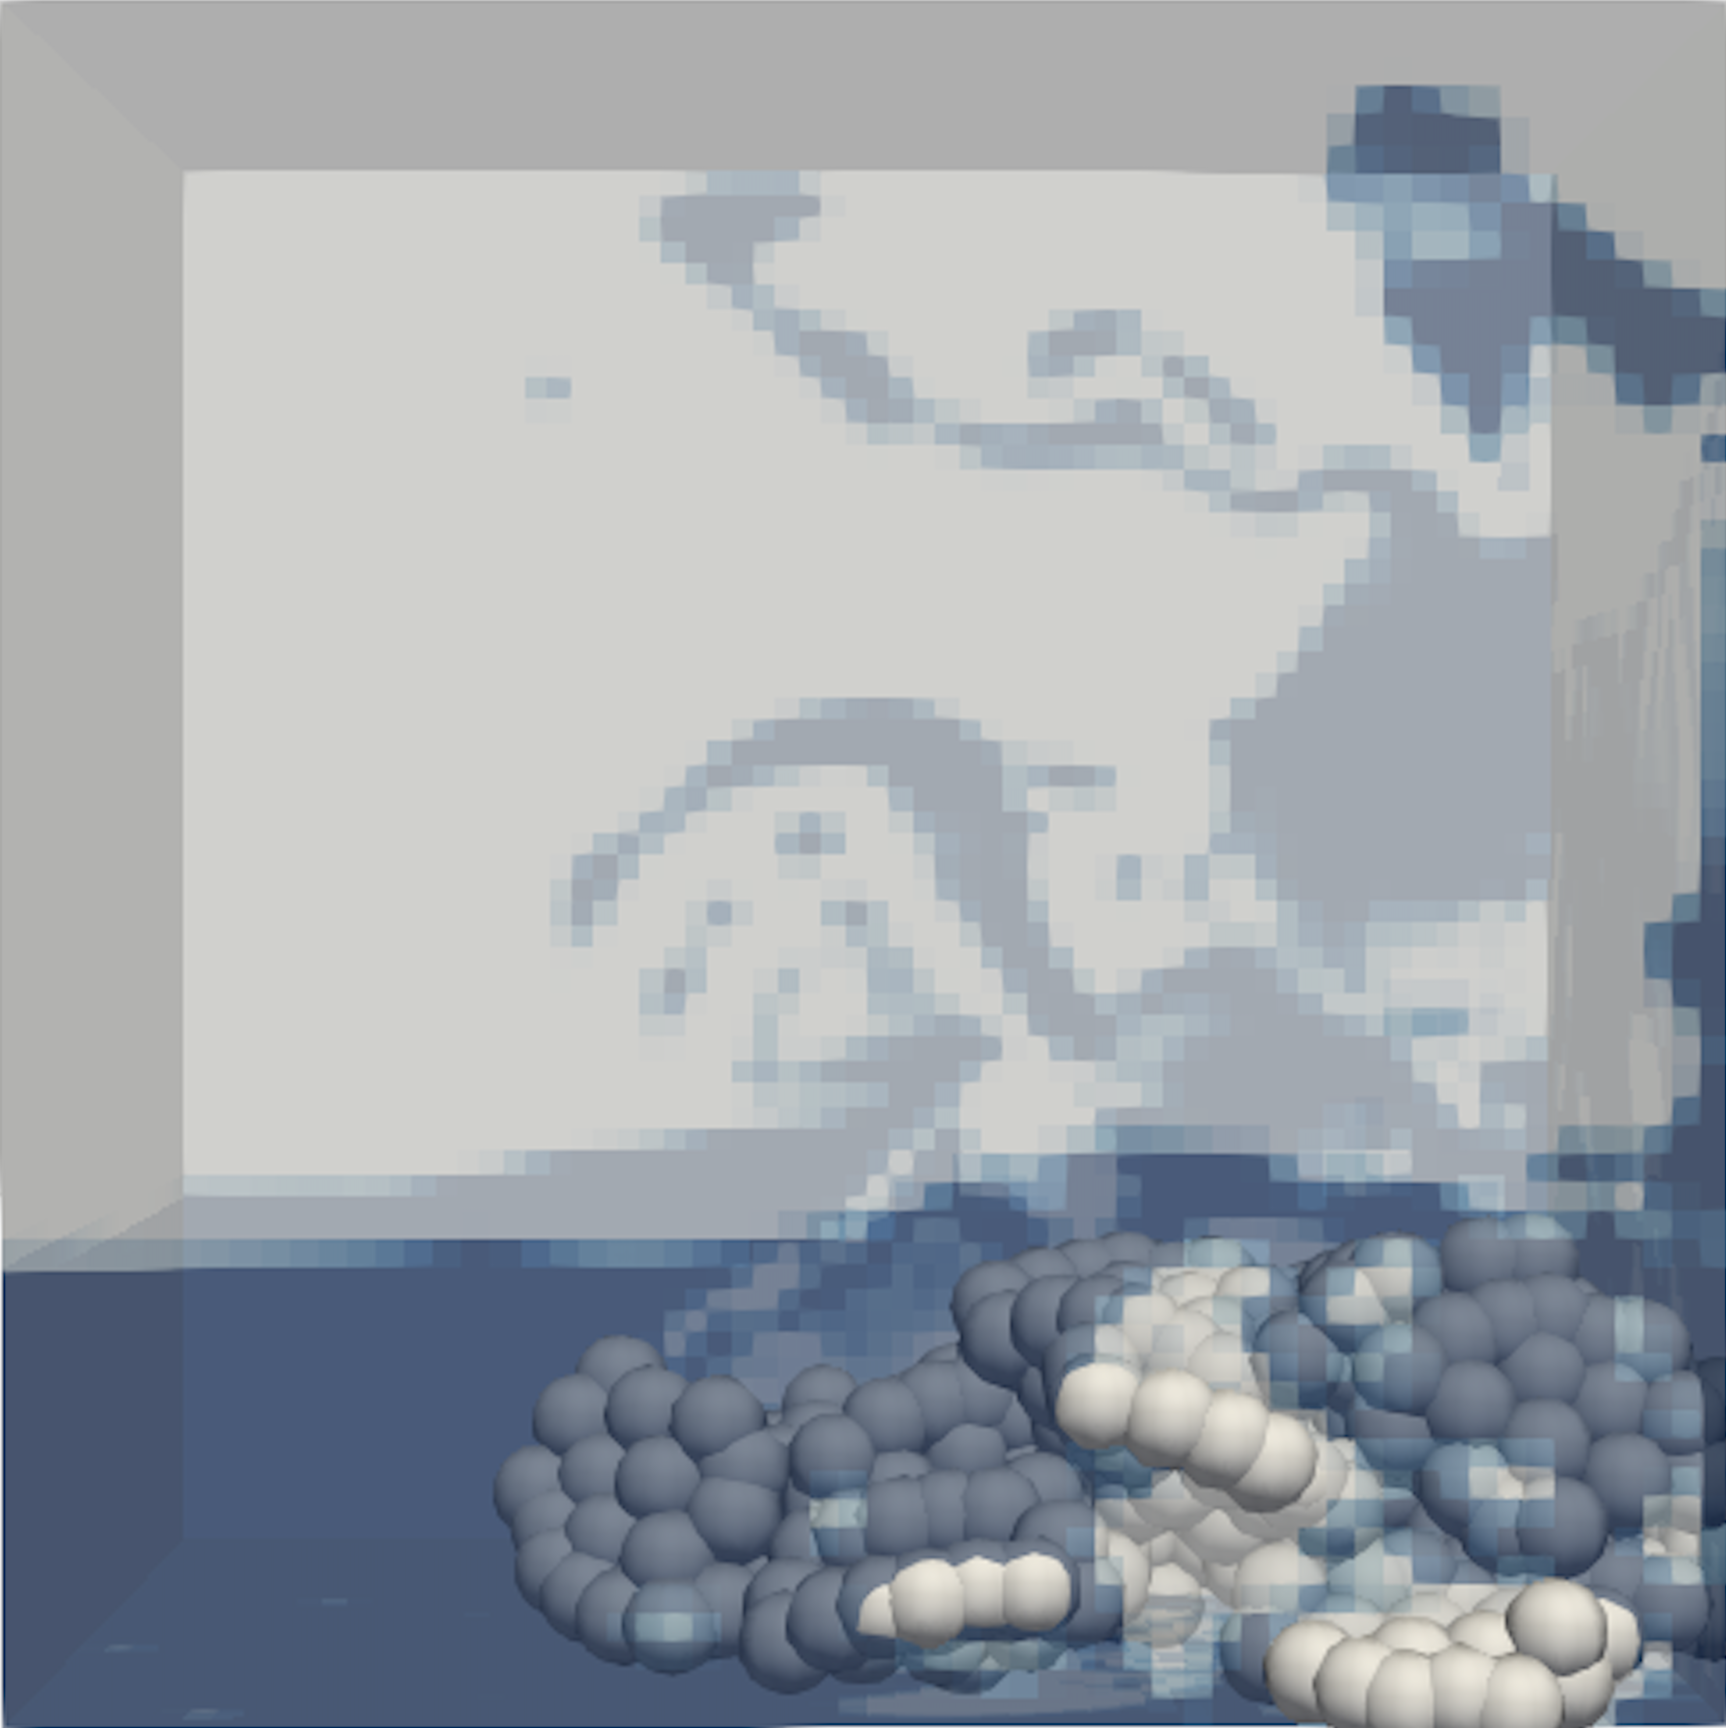
\includegraphics[width=\linewidth]{GWU_Thesis_Sarmakeeva/Images/chap4/landslide_6.png}
        \subcaption{0.3 sec}
    \end{minipage}
    \caption{Solid multi-spherical bodies interact with a collapsing column of liquid: a) clumps placement b) clumps moving under gravity force c) clumps fully covered by a body of fluid, fluid hits the right boundary of the domain d) clumps continue to move under fluid and gravity forces e) fluid flow continues to develop f) developing fluid flow and solid bodies rotation.}
    \label{fig:two-phase_exp_clumps}
\end{figure}

The simulations on Figures \ref{fig:two-phase_exp} and \ref{fig:two-phase_exp_clumps} show that the created numerical algorithm could be used for large-scale computations with a larger number of particles and handle complex multiphase flows with particle-fluid interactions, including the formation of clumps with various shapes. As the number of particles increases, the parallel domain decomposition approach can be further leveraged by distributing the computational load across a greater number of MPI processes, facilitating simulations at larger scales while maintaining numerical stability and reasonable computational times. The code leverages parallel computing capabilities through domain decomposition using the Message Passing Interface (MPI). The computational domain is decomposed into multiple subdomains, and each subdomain is assigned to a separate MPI process. In the case of these simulations, the simple domain decomposition method available in OpenFOAM was used. The MPI processes exchange boundary data at the interfaces between neighboring subdomains, enabling efficient parallel execution of the simulations. The code used for particle simulation \cite{LIGGGHTS} includes the possibility to use a number of clumps of different shapes, which also could better approximate real-world problems.

\begin{table}[H]
    \centering
    \caption{Computational time for multiple clump simulation.} \label{table4-chap4}
    \begin{tabular}{lr}
        \toprule
        \hline
       Number of processors     & Time (sec)\\
        \hline
        \midrule
        16 processors &  4500 sec \\
        32 processors &   2580 sec\\
        64 processors &   1320 sec\\
                                \hline
        \bottomrule
     \end{tabular}
\end{table}
The computational performance and parallel scalability of the developed solver were evaluated through multiple clump simulations with varying numbers of processors. Table~\ref{table4-chap4} presents the computational times for these simulations, demonstrating the effectiveness of parallel processing. As the number of processors increases from 16 to 32 and further to 64, a significant reduction in computational time is observed, indicating the solver's ability to leverage additional computational resources effectively.

%Speedup for 32 processors (N_max = 32) compared to 16 processors:
%S_32 = T_16 / T_32 = 4500 sec / 2580 sec = 1.74
%Speedup for 64 processors (N_max = 64) compared to 16 processors:
%S_64 = T_16 / T_64 = 4500 sec / 1320 sec = 3.41
%Parallel Efficiency = (Speedup * N_min / N_max) * 100%

\begin{figure}[H]
    \centering
    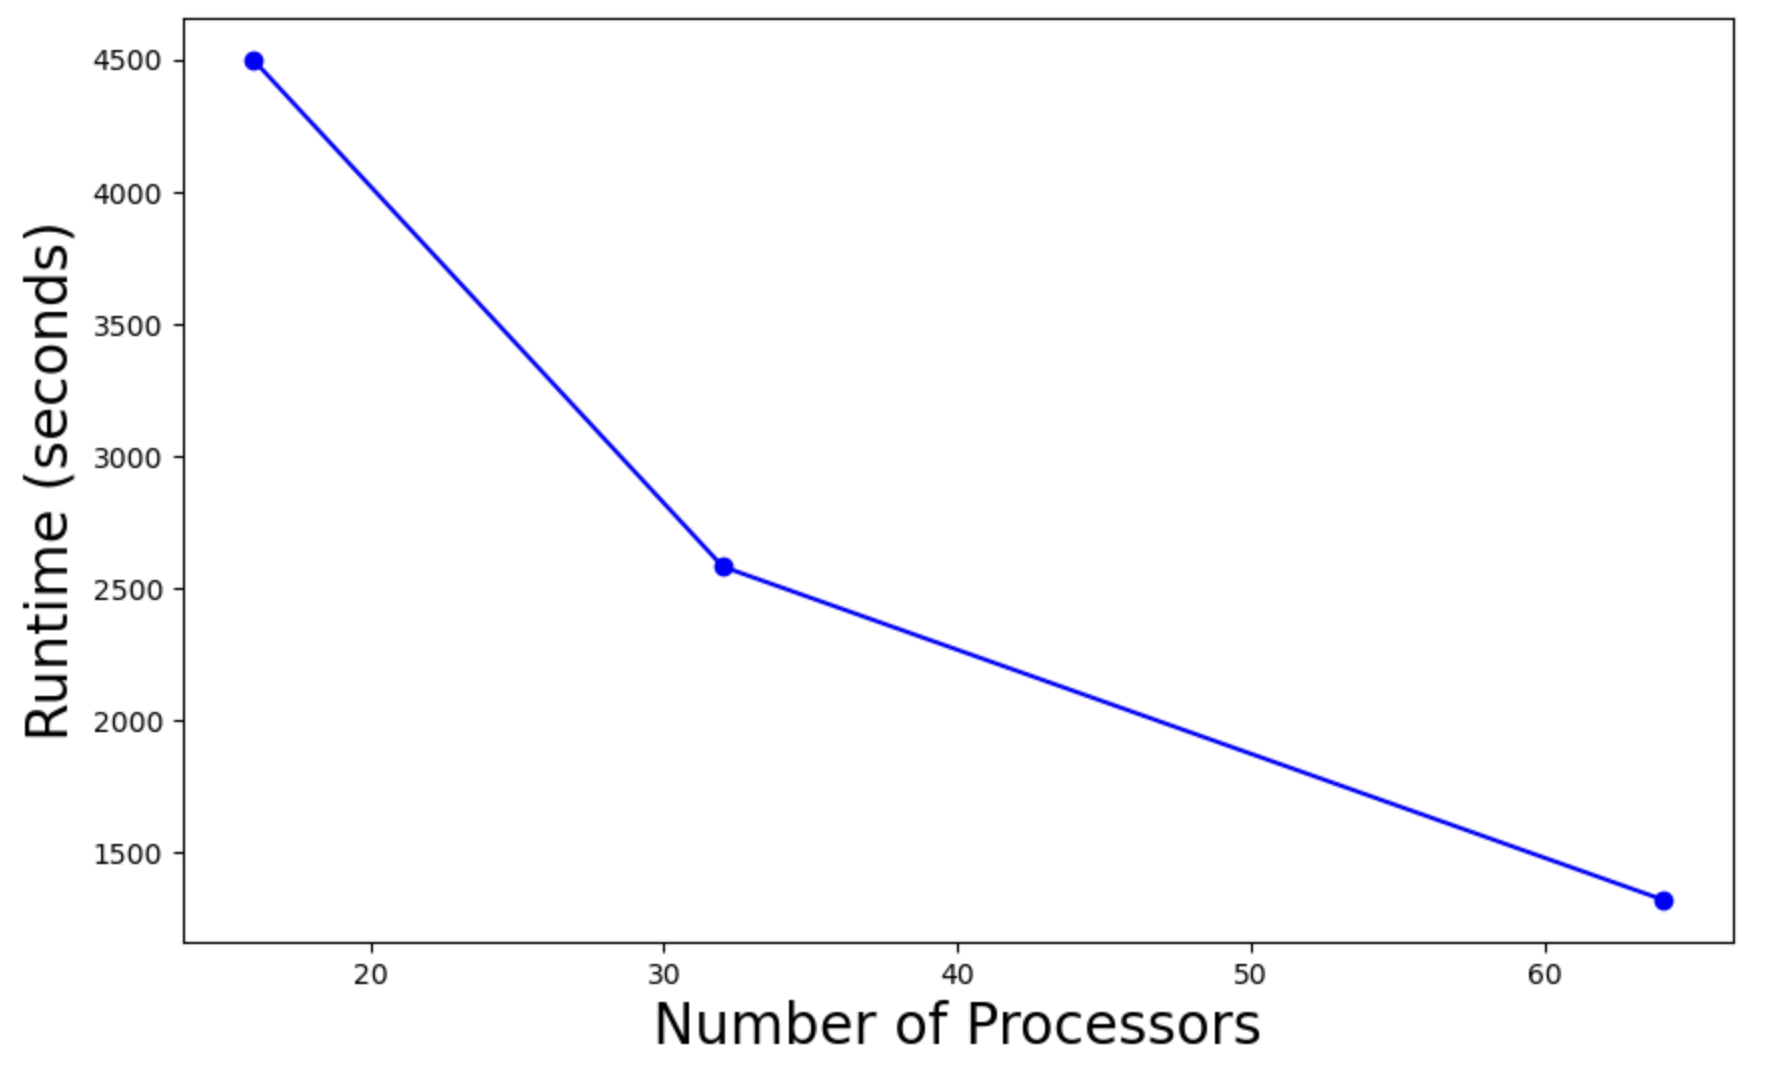
\includegraphics[width=15cm]{GWU_Thesis_Sarmakeeva/Images/chap3/parallel_runtime.png}
    \caption{Runtime (in seconds) versus number of processors for the experiment of solid multi-spherical bodies interacting with a collapsing column of liquid. }
    \label{fig:runtime}
\end{figure}

The parallel efficiency, a metric that quantifies the utilization of computational resources in parallel computing, was calculated for the 32 and 64 processor cases, using the 16 processor case as the baseline. The results show that the parallel efficiency is approximately 87\% when using 32 processors and 85.25\% when using 64 processors. These high parallel efficiency values, above the generally accepted threshold of 80\%, indicate good scalability and efficient utilization of the computational resources.

To calculate parallel efficiency we used formula:
$$\epsilon = S_p * \frac {N_{min}}{N_{max}}$$
where $S_p$ is speedup, $N_{min}$ and $N_{max}$ number of processors, since the option to run solver sequentially is not available.

However, it is worth to notice that a slight decrease in parallel efficiency is observed as the number of processors increases from 32 to 64. This issue could be explored in further works using profiling tools to understand the origin of overhead and potential load imbalance associated with distributing the workload across a larger number of processors. Nonetheless, the overall parallel performance showcases the solver's capability to handle large-scale simulations involving multiple clumps and particle-fluid interactions. These results show the benefits of parallel computation for the developed solver.

\section{Discussion}

%The initial goal of this work was to develop a tool that could be used for the simulation of landslides in coastal areas. To do so, we need to figure out methods suitable for this type of problem based on open-source code, then implement, verify, validate, and then test it. This is a nontrivial task and requires significant work. Validation and verification showed that the solver works as we suppose. Based on that, we run simulations testing the solver in more detail. We tested on bouncing body simulation, which showed stable results. Then we ran the simulation with multispherical bodies interaction and fluid with a developed solver, showing that it could handle complex interactions between solid and liquid phases effectively and the dynamics of multiple solid bodies. This capability is important for accurately simulating real-world scenarios such as landslides, sediment transport, and other particulate flow problems. The solver can manage geometrical complexities, as seen in the last simulation in Figure \ref{fig:two-phase_exp_clumps}. It can track the motion and interaction of bodies with non-uniform shapes through the fluid, which involves complex boundary conditions and potentially non-linear material behavior. The solver is effective for parallel computations by the decreased computation times with increased processor counts, as shown in Table \ref{table4-chap4}. Documentation for the solver is available online \ref{sarmakeeva_multiphaseIB}, as well as detailed documentation.

The primary objective of this study was to create a robust simulation tool which could be used for analyzing landslide phenomena in coastal environments. This endeavor required identifying and implementing suitable methods and leveraging open-source code as a foundational framework. The complexity of this task necessitated a comprehensive approach encompassing implementation, verification, validation, and extensive testing.

We run a series of simulations to examine the solver's capabilities. Initial tests involving the simulation of a bouncing body yielded numerical accuracy and achieved convergence even in cases with large deformations, or complex geometries, affirming the solver's reliability. Progressing further, we conducted simulations incorporating multispherical bodies interacting within a fluid using our developed solver. These tests demonstrated the solver's adeptness in managing complicated interactions between solid and liquid phases. This proficiency is critical for the accurate representation of real-world phenomena such as landslides, sediment transport, and other scenarios involving particulate flows.

A significant aspect of our solver is its ability to handle geometric complexities. This is evidenced in our simulations (see Figure \ref{fig:two-phase_exp_clumps}), where the solver tracked the motion and interaction of irregularly shaped bodies within the fluid. Given the complex boundary conditions and potential non-linear material behavior encountered in such simulations, this capability is crucial. 

%The solver code is accessible online \cite{github_solver} with post-processing data.

Moreover, our solver exhibits good scalability in parallel computing environments. We observed a reduction in computation times from 4500 sec to 2580 sec for 16 and 32 processors and to 1320 sec of computational time for the simulation of 64 processors for the experiment of solid multi-spherical bodies and two-phase fluid as detailed in Table \ref{table4-chap4}. This scalability is particularly beneficial for handling the computationally intensive tasks associated with fluid-solid interaction simulations.

 





